%Report template

\documentclass[10pt,a4paper]{amsart}

% Class options



\usepackage[utf8]{inputenc}
\usepackage{enumitem}
%\usepackage[latin1]{inputenc}
\usepackage[T1]{fontenc}
\usepackage{graphicx}
\usepackage{latexsym}
\usepackage{amsmath,amssymb, amsfonts, amsthm, stmaryrd, enumitem, mathtools}
\usepackage{ifpdf}
%\usepackage{natbib}
%\usepackage{mathabx} % bigtimes
\usepackage{mathrsfs} % mathscr
%\usepackage{subfig}
\usepackage{caption}
\usepackage{subcaption}
\usepackage{float}
\usepackage{color}
\usepackage{hyperref}
\usepackage{tikz}
\usetikzlibrary{snakes}
% plotting
\usepackage{pgfplots}
\pgfplotsset{compat=newest}
\pgfplotsset{every axis legend/.append style={
at={(0,0)},
anchor=north east}} 
%\everymath{\displaystyle}

% abbreviations
%\usepackage[intoc]{nomencl}
%\renewcommand{\nomname}{Notations}



% Modify top margin 
%\setlength{\topmargin}{-15mm}

% Theorems, definitions...
\usepackage{amsthm}
\usepackage{bbm}

\newtheoremstyle{exampstyle}
{15pt} % Space above
{15pt} % Space below
{} % Body font. Remove itshape if want texts of theorems normal and not in italics
{} % Indent amount
{\bfseries} % Theorem head font
{.} % Punctuation after theorem head
{.5em} % Space after theorem head
{} % Theorem head spec (can be left empty, meaning `normal')

\theoremstyle{exampstyle}

\newtheorem{Theorem}{Theorem}
\newtheorem{Definition}{Definition}
\newtheorem{Lemma}{Lemma}
\newtheorem{Remark}{Remark}
\newtheorem{Example}{Example}
\newtheorem{Corollary}{Corollary}
\newtheorem{Proposition}{Proposition}
%\newtheorem{Notation}{Notation}
\newenvironment{Proof}{\noindent{\textit{Proof.}}}{%
\hspace*{\fill}$\Box$\par\vskip2ex}
\newcommand{\bspend}{%
\hspace*{\fill}$\blacktriangleleft$\par\vskip2ex}
\newcommand{\bewend}{%
\hspace*{\fill}$\Box$\par\vskip2ex}

%\newtheorem{Theorem}[Theorem]{Theorem}
%\newtheorem{Definition}[Theorem]{Definition}
%\newtheorem{Lemma}[Theorem]{Lemma}
%\newtheorem{Remark}[Theorem]{Remark}
%\newtheorem{Example}[Theorem]{Example}
%\newtheorem{Corollary}[Theorem]{Corollary}
%\newtheorem{Proposition}[Theorem]{Proposition}
%\newtheorem{Notation}{Notation}
%\newenvironment{Proof}{\noindent{\textit{Proof.}}}{%
%\hspace*{\fill}$\Box$\par\vskip2ex}
%\newcommand{\bspend}{%
%\hspace*{\fill}$\blacktriangleleft$\par\vskip2ex}
%\newcommand{\bewend}{%
%\hspace*{\fill}$\Box$\par\vskip2ex}

\newtheoremstyle{exampnotations}
{15pt} % Space above
{15pt} % Space below
{} % Body font. Remove itshape if want texts of theorems normal and not in italics
{} % Indent amount
{\bfseries} % Theorem head font
{.} % Punctuation after theorem head
{.5em} % Space after theorem head
{} % Theorem head spec (can be left empty, meaning `normal')

\theoremstyle{exampnotations}  
\newtheorem{Notation}{Notation}

\usepackage{caption}

\usepackage{newclude}

\usepackage[final]{pdfpages}

\usepackage{fancyhdr}
\fancyhead{}
\fancyhead[RO]{\slshape \rightmark}
%\fancyhead[LE]{\slshape \leftmark}

%\allowdisplaybreaks
% instead: single \displaybreak in align-environment

\usepackage{hyperref}
%\hypersetup{
% colorlinks,
% citecolor=black,
% filecolor=black,
% linkcolor=black,
% urlcolor=black
%}

% macros
\newcommand{\rpos}{\mathbb{R}_\geq}
\newcommand{\Z}{\mathbb{Z}}
\newcommand{\R}{\mathbb{R}}
\newcommand{\N}{\mathbb{N}}
\newcommand{\E}{\mathbb{E}}
\newcommand{\kn}{\kappa_n}
\newcommand{\pl}{\left( \left\{ }
\newcommand{\pr}{ \right\} \right) }
\newcommand{\supt}{\sup_{0\leq t \leq T}}
\newcommand{\il}{\left( } % integrals
\newcommand{\ir}{\right) }
\newcommand{\Il}{\Bigg(} % integrals
\newcommand{\Ir}{\Bigg)}
\newcommand{\el}{\left[ }
\newcommand{\er}{\right] }
\newcommand{\El}{\Bigg[ }
\newcommand{\Er}{\Bigg] }
\newcommand{\rl}{\left(}
\newcommand{\rr}{\right)}
\newcommand{\Rl}{\Bigg(}
\newcommand{\Rr}{\Bigg)}
\newcommand{\vl}{\left|}
\newcommand{\vr}{\right|}
\newcommand\floor[1]{\lfloor#1\rfloor}
\newcommand\ceil[1]{\lceil#1\rceil}
\newcommand{\indep}{\rotatebox[origin=c]{90}{$\models$}}


%\makenomenclature

% Hyphenation
\hyphenation{Lip-schitz}
\hyphenation{sto-chas-tic}
\hyphenation{nu-me-ri-cal}
\hyphenation{appro-xi-ma-tion}
\hyphenation{accor-ding}
\hyphenation{mathematics}
\hyphenation{in-equa-li-ty}
\hyphenation{in-equa-li-ties}
\hyphenation{mea-sura-bi-li-ty}
\hyphenation{Brownian}
\hyphenation{Example}
\hyphenation{si-mu-la-tion}
\hyphenation{si-mu-la-tions}

% Appendices
%\usepackage[toc,page]{appendix}



% Colours
\definecolor{dark1}{RGB}{27, 158, 119}
\definecolor{dark2}{RGB}{217, 95, 2}
\definecolor{dark3}{RGB}{117, 112, 179}
\definecolor{dark4}{RGB}{231, 41, 138}  

%\usepackage{chngcntr}
%\counterwithout{footnote}{chapter}

\newcommand{\vertiii}[1]{{\left\vert\kern-0.25ex\left\vert\kern-0.25ex\left\vert #1 \right\vert\kern-0.25ex\right\vert\kern-0.25ex\right\vert}}

%\usepackage{tocloft}
%\setlength\cftbeforefigskip{\cftbeforechapskip}
%\setlength\cftbeforetabskip{\cftbeforechapskip}

\begin{document}
\title{Continuum Line-of-Sight Percolation on Poisson-Voronoi Tessellations}
\author[Q. Le Gall]{Quentin Le Gall}
\address{Orange Labs Networks, 44 avenue de la République 92320 Ch\^atillon}
\email{quentin1.legall@orange.com}
\author[B. B\l{}aszczyszyn] {Bart\l{}omiej B\l{}aszczyszyn}
\address{Inria - \MakeUppercase{ens}, 2 rue Simone Iff CS42112 75589 Paris Cedex 12}
\email{bartek.blaszczyszyn@ens.fr }
\author[E. Cali]{\'Elie Cali}
\address{Orange Labs Networks, 44 avenue de la République 92320 Ch\^atillon}
\email{elie.cali@orange.com}
\author[T. En-Najjary]{Taoufik En-Najjary}
\address{Orange Labs Networks, 44 avenue de la République 92320 Ch\^atillon}
\email{taoufik.ennajjary@orange.com}
\maketitle
\tableofcontents

\begin{abstract}
   In this work, we introduce a new model for continuum line-of-sight percolation in a random environment given by a Poisson Voronoi tessellation. The edges of this tessellation are the support of a Cox process, while the vertices are the support of a Bernoulli process. Taking the superposition $Z$ of these two processes, two points of $Z$ are linked by an edge if and only if they are sufficiently close and located on the same edge of the supporting tessellation. We study the percolation of the random graph arising from this construction and prove that a subcritical phase as well as a supercritical phase exist under %sufficiently 
   general assumptions. We also give numerical estimates of the critical parameters of the model. Our model can be seen as a good candidate for modelling telecommunications networks in a random environment with obstructive conditions for signal propagation.  
\end{abstract}
\section{Introduction}
\subsection{Background and motivation}
Bernoulli bond percolation, introduced in the late fifties by Boradbent and Hammersley \cite{broadbent1957percolation}, is one of the simplest mathematical models featuring phase transition. Since then, this model has been generalized in many different ways, making percolation theory a broader and still very active research topic today. 
\\ \indent Since the seminal work~\cite{gilbert1961random} of Gilbert, random graphs have been a key mathematical tool for the modelling of telecommunications networks. Good connectivity of the network is then interpreted by percolation of its associated connectivity graph. Over the years, Gilbert's original model has been refined and lots of mathematical models for telecommunications networks are now available in the literature.
\\ \indent In our previous work~\cite{LeGal1904:Influence}, we introduced and numerically studied a new mathematical model for modelling telecommunications networks in obstructive urban environments: we think of the urban network as being supported by a haphazard system of streets, modelled as a Poisson Voronoi tessellation (PVT) $S$. The edges of $S$ are the support of a Cox process modelling users of the network, and the vertices of $S$ are the support of a Bernoulli point process modelling relays. Considering the superposition of these %former
two point processes, say $Z$, we define a connectivity graph whose nodes are the points of $Z$ and where two points are joined by an edge if and only if they are sufficiently close \emph{and} located on the same edge of $S$. This is how we model obstructive conditions for signal propagation. Good connectivity of the network is then interpreted as percolation of the aforementioned connectivity graph. \\

\indent In this paper, we study this new model on a more theoretical approach. \emph{Our main findings are the following ones:}
\begin{itemize}
    \item \textbf{Minimal parameter for the Bernoulli process:} There exists a minimal parameter of the Bernoulli process $p=p^*$ under which percolation of the connectivity graph cannot happen with positive probability, regardless of all other parameters.
    \item Above the former threshold, two connectivity regimes exist:
    \begin{itemize}
        \item \textbf{Non-trivial subcritical phase :} If the connectivity range is not too large, then there exists a subcritical phase for percolation of the connectivity graph.
        \item \textbf{Non-trivial supercritical phase :} For sufficiently large $p<1$ and finite positive linear intensity of the Cox process, percolation happens with some positive probability.
    \end{itemize}
\end{itemize}
%\textbf{\textcolor{red}{Need to write with actual and concrete words what our results mean}}
 \vskip \baselineskip \emph{The rest of this paper is organised as follows:} We begin with recalling some related works in Subsection~\ref{Ss.Relatedworks}. Then, we present our network model and introduce convenient notations in Section~\ref{S.Model}. In Section~\ref{S.Results}, we state our theoretical results in more detail and proceed with their proofs. In Section~\ref{S.NumericalSimulations}, we present results of numerical simulations to illustrate our main mathematical results. Finally, we conclude and give perspectives for future work in Section~\ref{S.Conclusion}.
\subsection{Related works}
\label{Ss.Relatedworks}
In~\cite{gilbert1961random}, Gilbert introduced percolation in a continuum setting by considering a planar homogeneous Poisson point process where two points are joined by an edge if and only if they are separated by a distance gap less than a given threshold. %$R$ in the plane. 
This model has at the time been considered to be a good candidate for representing a telecommunications network, with the range of the stations being taken into account as a parameter. The Poisson case has now extensively been studied \cite{FnT1,meester_continuum_1996} and Gilbert's model has recently been extended to other types of point processes, among which sub-Poisson \cite{blaszczyszyn2010connectivity,blaszczyszyn2013clustering,blaszczyszyn2015clustering} , Ginibre \cite{ghosh2016continuum} and Gibbsian \cite{jansen2016continuum,stucki2013continuum}. 
\\ \indent The study of percolation processes living in random environments has only been considered recently and outlined that many standard techniques from Bernoulli or continuum percolation cannot be applied in a random environment setting.
%fail to carry over in a random environment setting
%Recent results on random unimodular graphs \cite{beringer2017percolation} confirmed this fashion 
As a matter of fact, new tools and techniques had to be introduced. In this regard, the paper from Bollob\'as and Riordan \cite{bollobas2006critical} on the threshold of Voronoi percolation in the plane is pioneering. Later on, \cite{ahlberg2016quenched,tassion2016crossing} brought additional results concerning this model. Other percolation models \cite{vahidi1990first}, tessellations \cite{bollobas2008percolation} and other random graphs \cite{balister2008percolationknearest, balister2008percolation, beringer2017percolation} have also been considered. A more general study of Bernoulli and first-passage percolation on random tessellations has been conducted in \cite{ziesche2016bernoulli,ziesche2016first}. 
\\ \indent A natural extension of Gilbert's model in a random environment setting is obtained by considering a Cox point process, i.e. a Poisson point process with a random intensity measure. Percolation of Gilbert's model in such a setting has theoretically been studied for the first time in \cite{hirsch2018continuum}. %Numerical aspects of Gilbert's model for Cox processes with applications to telecommunications networks have then been explored in \cite{cali2018percolation}. Only very recently, SINR percolation for Cox processes has been investigated in \cite{tobias2018signal}.
\\ \indent In Gilbert's original model, connectivity between two network nodes only depends on their mutual Euclidean distance. This assumption has proven to be quite simplistic for the modelling of real telecommunications networks, where physical phenomena such as interference, fading or shadowing are at stake, making connectivity between two nodes to occur depend on other factors. As a matter of fact, other extensions of Gilbert's work have been considered for a more accurate modelling of telecommunications networks. In particular, percolation of the signal-to-interference-plus-noise ratio (SINR) model, where a connection between a pair of points does not only depend on their relative distance anymore but also on the positions of all other nodes of the network, has theoretically been studied in \cite{dousse2006percolation}. SINR percolation for Cox point processes has only been explored very recently \cite{tobias2018signal}. On a more applied perspective, random tessellations have turned out to yield good fits of real street systems, as has been proven in \cite{gloaguen2006fitting}. Percolation thresholds of the Gilbert graph of Cox processes supported by random tessellations have numerically been investigated in \cite{cali2018percolation}, yielding other interesting applications for telecommunication networks. 
\\ \indent Recently, mathematical models of so-called \emph{line-of-sight} (LOS) networks have been introduced, modelling telecommunication networks in environments with regular obstructions, such as large urban environments or indoor environments. Nodes of the network are then connected when they are sufficiently close %to one another
and when they have line-of-sight access to one another, in other words if no physical obstacle stands between them. In \cite{frieze2009line}, asymptotically tight results on $k$-connectivity of the connectivity graphs arising from such models are studied. Bollobàs, Janson and Riordan \cite{bollobas2009line} extend these results by introducing a line-of-sight site percolation model on the discrete square lattice $\mathbb{Z}^{2}$ and the two-dimensional $n$-torus $\left[0 \times n \right]^2$ and asymptotical results for the critical probability were derived as well. Interesting connections to Gilbert's continuum percolation model were also investigated. However, the study of line-of-sight percolation in a continuum setting with a random environment has not, %to the state of our knowledge, 
as far as we know, been studied yet. \\ \indent It is in light of these recent developments that we introduced a new percolation model for Cox processes supported by Poisson-Voronoi tessellations (PVT) in our previous work \cite{LeGal1904:Influence}. 
%, where two network nodes are connected if and only if they are sufficiently close and located on the same edge of the supporting PVT. We now investigate this new model on a more theoretical approach and will be interested in theoretical proofs which had to be postponed in our previous work.

%\subsection{Main findings} In our new model 
%introduced in \cite{LeGal1904:Influence}, 
%we consider the PVT $S$ generated by a stationary homogeneous planar Poisson point process. The edges of tessellation will be the support of a Cox point process \cite[Section 5.2]{chiu_stochastic_2013}, and the vertices of $S$ will be the support of a Bernoulli point process \cite[Section 2.2]{chiu_stochastic_2013}, whose atoms will ensure connectivity between adjacent edges of $S$. We then consider the superposition of these two point processes, say $Z$. Any two distinct points of $Z$ are joined by an edge if and only if they are located on the same edge of $S$ and their relative Euclidean distance is less than a given threshold. This defines a connectivity graph whose percolation regimes are studied in this paper. For this study, relevant parameters, to be properly defined in Section~\ref{S.Model}, are:
%\begin{itemize}
    %\item $\lambda$, the linear intensity of the Cox process $\lambda$ (i.e. the mean number of Cox points per edge of the PVT $S$)
    %\item $p$, the parameter of the Bernoulli process (i.e. the mean proportion of PVT vertices that are atoms of the Bernoulli process)
    %\item $r$, the connectivity range
%\end{itemize}

%\begin{itemize}
    %\item \textbf{Minimality condition:} There is a minimal parameter of the Bernoulli process below which the connectivity graph of our model does not percolate, regardless of all other parameters.
    %\item \textbf{Non-trivial sub-critical phase under certain conditions:} If the Bernoulli parameter exceeds the former threshold and if the connectivity threshold is sufficiently small, there is a non-trivial sub-critical phase for percolation of the connectivity graph.
   % \item \textbf{Non-trivial super-critical phase:} There is a non-trivial super-critical phase for percolation of the connectivity graph of our model
%\end{itemize}


\section{Model definition and main results}
\label{S.Model}
\subsection{Network model}
\label{Ss.NetworkModel}
Consider a probability space $(\Omega, \mathcal{F}, \mathbb{P})$ and state space $(\mathbb{R}^{2}, \mathcal{B}(\mathbb{R}^{2}))$, where $\mathcal{B}(\mathbb{R}^{2})$ is the usual Borel $\sigma$-algebra of $\mathbb{R}^{2}$. \\

Let $\lambda_{S} > 0$ and $X_{S}$ be a homogeneous planar Poisson point process (PPP) in the state space $\mathbb{R}^{2}$ with intensity $\lambda_S$. Consider the Poisson-Voronoi tessellation (PVT) $S$ associated with $X_S$. In particular, $S$ is stationary and isotropic. By analogy with a telecommunications network, $S$ will be called \emph{street system} from now onwards. Moreover, note that $S$ is  scale-invariant. %motion-invariant
%As a matter of fact, we assume $\lambda_S$ to be fixed throughout the rest of this paper by setting $\lambda_S = 1$.  \\
\\ \indent Denote by $E \coloneqq (e_{i})_{i \geq 1}$ the edge-set of $S$ and by $V \coloneqq (v_{i})_{i \geq 1}$ the vertex-set of $S$. Furthering the aforementioned analogy, the elements of $E$ (respectively $V$) will be called \emph{street segments} (respectively \emph{crossroads}). \\
\indent Let $\Lambda$ be the stationary random measure defined such that:
\begin{itemize}
\item $\mathbb{E} \Lambda \left[0,1\right]^{2} = 1$
\item $\Lambda(dx) = \nu_{1}(S \cap dx)$, where $\nu_{1}$ denotes the 1-dimensional Hausdorff measure of $\mathbb{R}^{2}$. In other words, for a Borel set $B \subset \mathbb{R}^2$, $\nu_{1}(S \cap B)$ is the total edge length of $S$ contained in  $B$ and so $\Lambda$ can be seen as a Lebesgue-like measure on the edges of $S$, rescaled in such a way that the total $\Lambda$-measure of a 1-area window is 1. \\
\end{itemize}


The users, equipped with mobile devices, are modelled by a Cox process $X^{\lambda}$ driven by the random intensity measure $\lambda \Lambda$. In other words, conditioned on a given realization of the street system $S$, $X^{\lambda}$ is a PPP with mean measure $\lambda \Lambda$. In particular, the number of users on a given street segment $e \in E$ is a Poisson random variable with mean $\nu_{1}(e)$ and the numbers of users on two disjoint subsets of $E$ are independent random variables. \\
\indent The relays (either representing physical antennas or additional users not modelled through $X^{\lambda}$) are modelled by a doubly stochastic Bernoulli point process $Y$ on the set of crossroads $V$ with parameter $p$, so that one can write:
%thinning of vertices of $S$ ?
\begin{equation*}
Y = \sum_{i} \mathbbm{1}_{\lbrace U_{i} \leq p \rbrace } \delta_{v_{i}},
\end{equation*}
where $U_{i} \;\substack{ \text{i.i.d.} \\ \sim} \; \mathcal{U}(0,1)$ and where $\delta_{x}$ denotes the Dirac measure at $x$. In other words, conditioned on $\Lambda$ (or, equivalently, $S$) each crossroad is retained (resp. erased) independently from all others with probability $p$ (resp. $1-p$). \\
\noindent Moreover, we also assume that the processes of users and of relays  are conditionnally independent given their random support, i.e. $X^{\lambda} \indep Y \, \vert \,  \Lambda$. We denote $Z \coloneqq X^{\lambda} \cup Y$ the superposition of users and relays. \\
%Then, conditioned on $\Lambda$, $Z$ has an independence property similar to the one of Poisson processes:
%\begin{Proposition}
%Given $\Lambda$, $Z$ has the complete independence property.
%\end{Proposition}
%\begin{Proof}
%Let $A, B \subset \mathbb{R}^{2}$ be Borel sets such that $A \cap B = \emptyset$. We need to show that $Z(A) \indep Z(B) \, \vert \, \Lambda$.
%\end{Proof}
%\vspace{2\baselineskip}

The key network parameters are:
\begin{itemize}
\item The user density $\lambda > 0$.
\item The relay proportion $p \in \left(0,1\right)$.
\item The connectivity range $r > 0$. \\
\end{itemize}

The network is then modelled by the \emph{connectivity graph} $\mathcal{G}_{p,\lambda,r}$ defined in the following way:
\begin{itemize}
\item $\mathcal{G}_{p,\lambda,r}$ is undirected.
\item The vertex set of $\mathcal{G}_{p,\lambda,r}$ is given by the points of $Z$.
\item The edge $Z_{i} \leftrightsquigarrow Z_{j}, i \neq j$ is drawn if and only if $Z_{i}$ and $Z_{j}$ are located on the \emph{same} street segment and of mutual Euclidean distance less than $r$. In other words:
\begin{equation}
\label{connectivity_mechanism}
\forall \, i \neq j, \: Z_{i} \leftrightsquigarrow Z_{j} \Leftrightarrow 
\left\{
\begin{array}{l}
\exists \, e \in E, \, Z_{i} \in e  \  \text{and} \  Z_{j} \in e \\
\lVert Z_{i} - Z_{j} \rVert \leq r
\end{array}
\right.
\end{equation}
\end{itemize}
\indent Figure~\ref{fig:Network} illustrates an example of a realization of our network model and of its connectivity graph in a bounded observation window. The blue lines represent the random environment (PVT) supporting the Cox process of users illustrated by red points. The Bernoulli process of relays is illustrated by the green points. Finally, possible connections are highlighted in orange and illustrate the connectivity mechanism given by~\eqref{connectivity_mechanism}.
\begin{figure}[h!]
\centering
    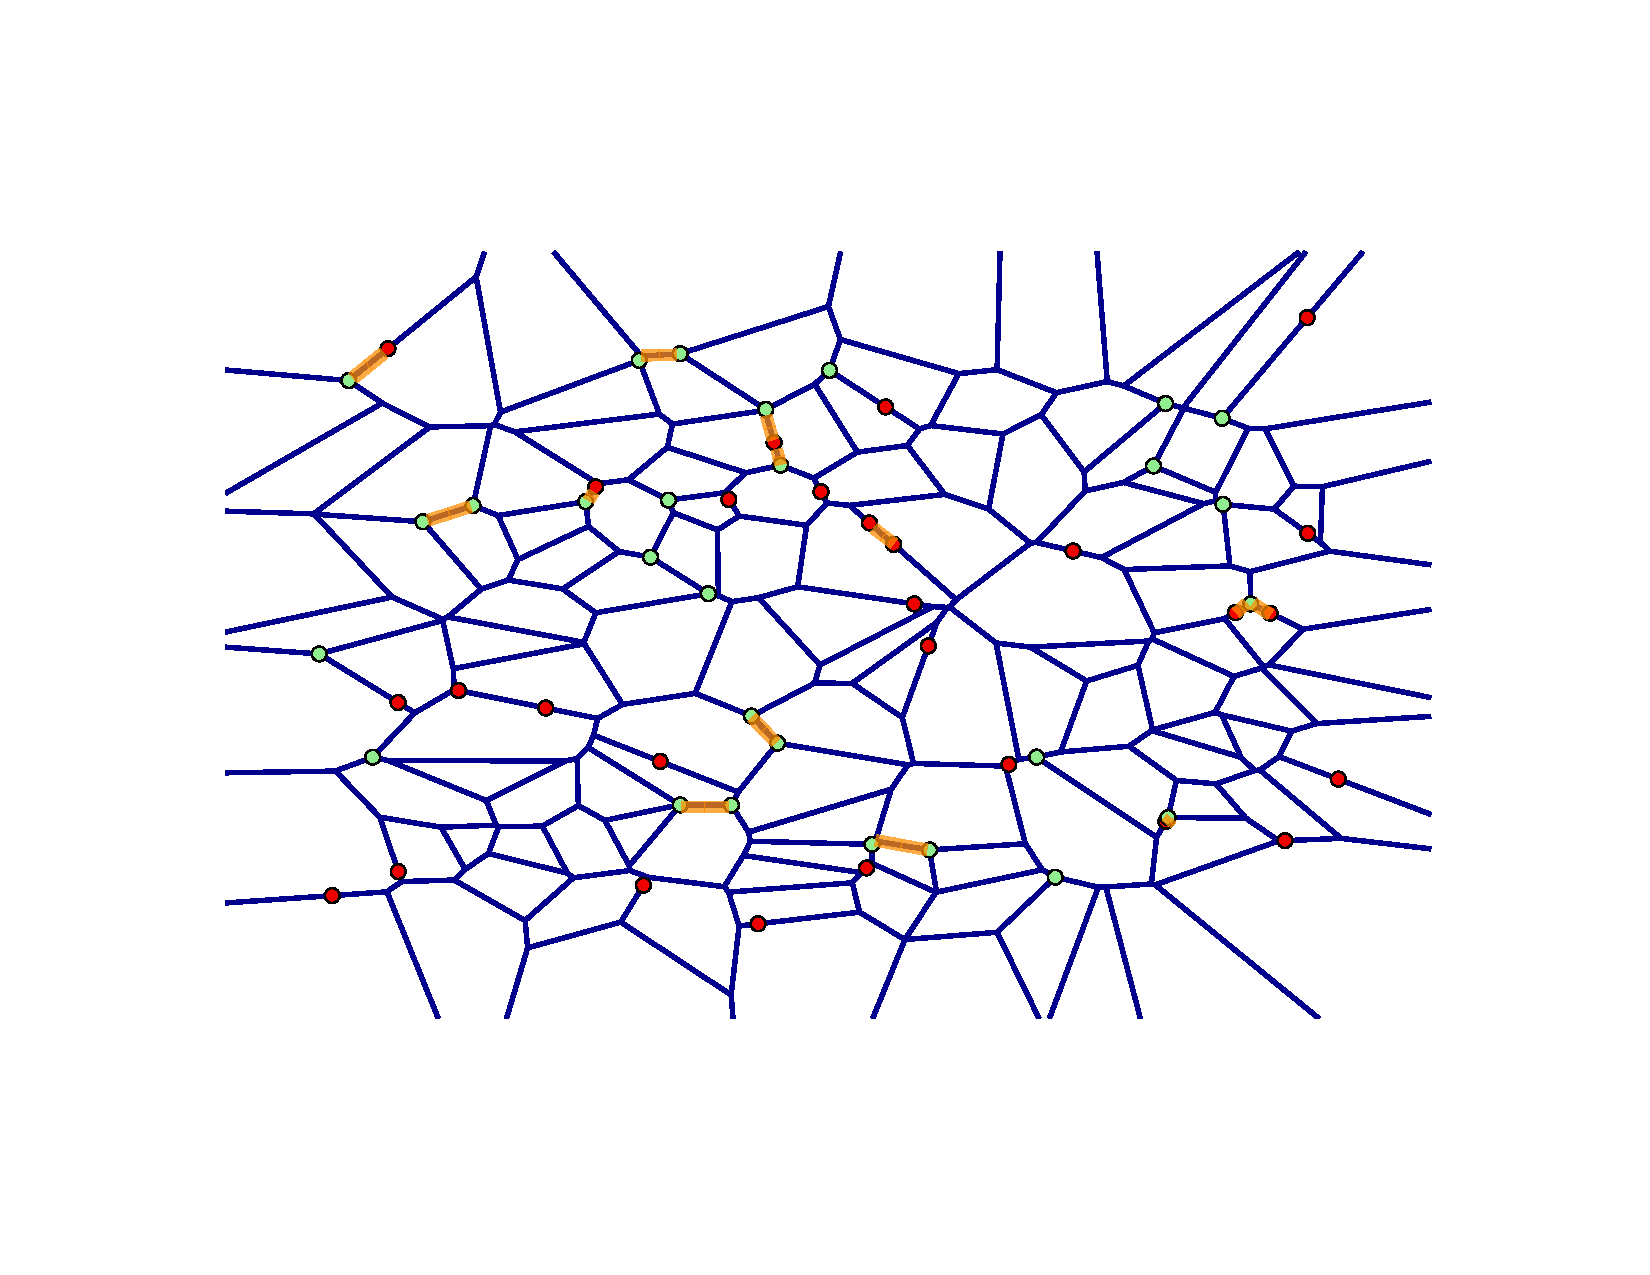
\includegraphics[width=0.6\linewidth]{Network.pdf}
    \caption{Illustration of a realization of the connectivity graph of our model for LOS networks supported by a random environment in a continuum setting.}
    \label{fig:Network}
\end{figure}

%\begin{Remark}
%The connectivity mechanism defined by \eqref{connectivity_mechanism} only allows for so-called line-of-sight (LOS) connections, which can be seen as a modelling of physical obstacles preventing connections to occur in all directions.
%\end{Remark}

\indent In this paper, our main concern is the percolation regime of the connectivity graph $\mathcal{G}_{p,\lambda,r}$. In other words, the main question we address is: Are there critical values of the parameters $(p,\lambda,r)$ for which percolation of $\mathcal{G}_{p,\lambda,r}$ occurs with positive probability?

%\paragraph*{Main question :} Percolation regime of the connectivity graph $\mathcal{G}_{p,\lambda,r}$? Are there critical values of the parameters $(p,\lambda,r)$ for which percolation of $\mathcal{G}_{p,\lambda,r}$ occurs with positive probability?

\subsection{Definitions and Notations}
We begin with introducing a few notations and definitions which will be useful for the purposes of our developments. \\


\indent For $A \subset \mathbb{R}^{2}$ and $B \subset \mathbb{R}^{2}$, we denote as customary the Euclidean distance between $A$ and $B$ by:
 $$\text{dist}(A,B) \coloneqq \inf \lbrace \lVert x - y \rVert_{2} , \,  x \in A, \,  y \in B \rbrace$$
\\

\indent For $x \in \mathbb{R}^{2}$, $n \in \mathbb{N} \setminus \lbrace 0 \rbrace$, we denote by $Q_n(x) \coloneqq x + \left[-n/2,n/2\right]^{2}$ the square of side $n$ centered at $x$. We note that this is exactly the definition of the closed ball with center $x$ and radius $n/2$ for the infinite norm of $\mathbb{R}^2$:
\begin{equation*}
    Q_n(x) = \lbrace y : \lVert y-x \rVert_{\infty} \leq n/2 \rbrace = \mathscr{B}(x,n/2)
\end{equation*}
For simplicity, whenever $n \in \mathbb{N} \setminus \lbrace 0 \rbrace$, we will write $Q_n$ to mean $Q_n(0)$. \\

\indent We will use the following convenient notation for the length of a street segment or a subset of street segment: let $e \in E$ and $s \subseteq e$. Then we denote the length of $s$ by $\vert s \vert$. \\

We will also need the concepts of \emph{stabilization} and \emph{essential asymptotic connectedness} given in \cite{hirsch2018continuum} for investigating spatial dependencies of random measures. \\
To that end, we denote by $\mathbf{M}$ the space of Borel measures on $\mathbb{R}^{2}$, equipped with the evalutation $\sigma$-algebra \cite[Section 13.1]{last2017lectures}, i.e. the smallest $\sigma$-algebra making the mappings $\mathbf{M} \ni \Xi \mapsto \Xi(B)$ measurable for all Borel sets $B \subset \mathbb{R}^{2}$. For a (possibly random) Borel measure $\mu$ on $\mathbb{R}^{2}$ and $A \subset \mathbb{R}^{2}$, we denote the restriction of $\mu$ to $A$ by $\mu_A(\cdot) \coloneqq \mu(A \cap \cdot)$. We also adapt the definition of the support of a measure as follows: let $\mu$ be a (possibly random) Borel measure on $\mathbb{R}^{2}$. The \emph{support} of $\mu$ is the following set:
$$\text{supp}(\mu) \coloneqq \lbrace x \in \mathbb{R}^{d} \, : \forall \varepsilon > 0, \,  \mu(Q_{\varepsilon}(x)) > 0 \rbrace$$


The concept of stabilization for investigating spatial dependencies of random measures has been introduced in many different ways in the literature. We use the same definition as the one introduced in~\cite{hirsch2018continuum}:
\begin{Definition}\cite[Definition 2.3]{hirsch2018continuum}
\label{Def.stabilizing}
A random measure $\Xi$ on $\mathbb{R}^{2}$ is called \emph{stabilizing} if there exists a random field of stabilization radii $R = \lbrace R_{x} \rbrace _{x \in \mathbb{R}^{2}}$ defined on the same probability space as $\Xi$ such that:
\begin{enumerate}[label = (\arabic*)]
\item $(\Xi,R)$ are jointly stationary
\item $\displaystyle \lim_{n \uparrow \infty} \mathbb{P}\left(\sup _{y \in Q_{n} \cap \mathbb{Q}^{2}} R_{y} < n\right) = 1$
\item for all $n \geq 1$, the random variables 
$$ \left\lbrace f\left(\Xi_{Q_{n}(x)}\right)\mathbbm{1}\left\lbrace \sup_{y \in Q_{n}(x) \cap \mathbb{Q}^{2}} R_{y} < n \right\rbrace \right\rbrace _{x \in \varphi}$$
are independent for all bounded measurable functions $$f : \mathbf{M} \to \left[0, +\infty \right)$$ and finite $\varphi \subset \mathbb{R}^{2}$ such that $\forall \, x \in \varphi, \, \text{dist}(x, \varphi \setminus \lbrace x \rbrace ) > 3n$.
\end{enumerate}
\end{Definition}
\begin{Remark}
Throughout the rest of this paper, we assume the random variables $(R_x)_{x \in \mathbb{R}^{2}}$ to be $\Lambda$-measurable, as has been done by the authors of \cite{hirsch2018continuum}.
%How do we deal with that in the end?
\end{Remark}
%\begin{Remark}
%In the above definition, the random field of stabilization radii $R = \lbrace R_{x} \rbrace _{x \in \mathbb{R}^{2}}$ may not be unique, i.e. a random measure can be stabilizing for more than one field of stabilization radii.
%\end{Remark}
%\begin{Remark}
%Let $b > 0$ and assume that $\Xi$ is $b$-dependent, i.e. $$\forall A,B \subset \mathbb{R}^{d}, \, \text{dist}(A,B) > b \Rightarrow \Xi_{A} \indep \Xi_{B}$$ Then $\Xi$ is stabilizing. 
%\end{Remark} 

\indent We slightly modify the definition of asymptotical essential connectedness given in~\cite{hirsch2018continuum} for the sake of simplicity and use the following definition:
\begin{Definition} %\cite[Definition 2.5]{hirsch2018continuum}
\label{Def.eac}
Let $\Xi$ be a random measure. Then $\Xi$ is \emph{essentially asymptotically connected} if there exists a random field $R = \lbrace R_{x} \rbrace_{x \in \mathbb{R}^{d}}$ such that $\Lambda$ is stabilizing for $R$ and if for all $n \geq 1$, whenever $\displaystyle \sup_{y \in Q_{2n} \cap \mathbb{Q}^{2}} R_{y} < n/2$, the following assertions are satisfied:
\begin{enumerate}[label = (\arabic*)]
\item $\text{supp}(\Xi_{Q_{n}}) \neq \emptyset$
\item $\text{supp}(\Xi_{Q_{n}})$ is contained in a connected component of $\text{supp}(\Xi_{Q_{2n}})$
\end{enumerate}
\end{Definition}

As a matter of fact, we introduce the following notation for convenience: for $x \in \mathbb{R}^{2}$ and $n \in \mathbb{N}\setminus \lbrace 0 \rbrace$ we denote:
$$R(Q_n(x)) \coloneqq \sup_{y \in Q_n(x) \cap \mathbb{Q}^{2}} R_y$$
whenever $\Xi$ is a stabilizing random measure for the stabilization field $R = \lbrace R_x \rbrace _{x \in \mathbb{R}^{2}}$. \\

The following result is stated in~\cite[Example 3.1]{hirsch2018continuum} for a slightly modified version of Definition~\ref{Def.eac}. It is easy to check that it adapts in our case as follows:

\begin{Proposition}
Let $\Lambda = \nu_{1}(S \cap dx)$, where $S$ is the PVT generated by an homogeneous stationary Poisson point process. Then $\Lambda$ is stabilizing and essentially asymptotically connected for the following stabilization field:
$$\forall x \in \mathbb{R}^{2}, \, R_x = \inf \lbrace \lVert x - X_{S,i} \rVert , \, X_{S,i} \in X_{S} \rbrace,$$
where $X_S$ is the PPP having generated $S$.
\end{Proposition}




\indent Finally, as is customary in any percolation problem, we need to define concepts of openness and closedness for the study of connected components. In our model, these definitions are adapted to crossroads and parts of street segments (possibly the whole street segments themselves) as follows:
%opennness and closedness? What's the therm?

\begin{Definition}[Open/Closed crossroad]
\label{Def.open/crossroad}
Say a crossroad $v \in V$ is \emph{open} if it is an atom of the point process $Y$, i.e. $Y(\lbrace v\rbrace) = 1$, or, equivalently:
\begin{equation*}
   \exists \,  i \geq 1, v=v_i \: \text{and } U_i \leq p
\end{equation*}
Say $v$ is \emph{closed} if it is not open, i.e. $Y(\lbrace V_i \rbrace) = 0$, or, equivalently:
\begin{equation*}
   \exists \,  i \geq 1, v=v_i \: \text{and } U_i > p
\end{equation*}
\end{Definition}

\begin{Definition}[Open/Closed street segment]
\label{Def.open/closed/subcritical}
Let $e \in E$ be a street segment and let $\emptyset \neq s \subseteq e$ be a non-empty subset of $e$.\\ Say $s$ is \emph{open} if either of the two following set of conditions are satisfied:
\begin{enumerate}
\item $\vert s \vert \leq r$
\vspace{.2 cm}
\item[]\textbf{OR}
\vspace{.2 cm}
\item $\left\{
\begin{array}{l}
\vert s \vert > r \\
\forall c \subset s, \, (\vert c \vert = r \; , c \text{ connected and} \; c  \; \text{topologically closed} )\Rightarrow X^{\lambda}(c) \geq 1
\end{array}
\right.$
\end{enumerate}
Say $s$ is \emph{closed} if $s$ is not open, i.e.: \\
 $\left\{
\begin{array}{l}
\vert s \vert > r \\
\exists \, c \subset s, \; \text{such that} \, \vert c \vert = r \; ,c \text{ connected,} \; c  \; \text{topologically closed} \; \text{and} \,  X^{\lambda}(c) = 0
\end{array}
\right.$
\end{Definition}

\section{Results}
\label{S.Results}
Our results concern the phase transition of the connectivity graph corresponding to the model presented in Section~\ref{Ss.NetworkModel} as well as a minimality condition on $p$ to make percolation to occur possible. Namely, we have the following:

\begin{Theorem}[Minimality condition on $p$]
\label{Thm.minimality}
Let $p^*$ be the Voronoi site percolation threshold (a theoretical estimate is given in~\cite{neher2008topological} and a numerical one is given in~\cite{becker_percolation_2009}). Let $p < p^*$. Then, for all $\lambda > 0$ and $r >0$, the connectivity graph $\mathcal{G}_{p,\lambda,r}$ does not percolate with probability 1.
\end{Theorem}

Concerning the sub-critical phase, we have the following:
\begin{Theorem}[Existence of a non-trivial sub-critical phase]
\label{Thm.subcritical}
Assume $p=1$. %Then there exists a minimal threshold $r_{0} > 0$ satisfying the following property: whenever $0<r < r_0$, we have
For given $r>0$, denote by $\lambda_c(r)$ the critical user density required for percolation of the connectivity graph $\mathcal{G}_{1,\lambda,r}$:
\begin{equation*}
    \lambda_c(r) \coloneqq \inf \lbrace \lambda > 0 : \, \mathbb{P}(\mathcal{G}_{1, \lambda, r} \; \text{percolates}) > 0 \rbrace
\end{equation*}
Then, denoting $ r_0 \coloneqq \sup \lbrace r > 0 : \, \lambda_c(r) > 0 \rbrace$, we have that $0 < r_0 < \infty$. \\
In other words, if the connection radius is not too large, there exists a subcritical phase for percolation of the connectivity graph when all crossroads are equipped with a relay.
\end{Theorem}

A straightforward consequence of Theorem~\ref{Thm.subcritical} is the following:

\begin{Corollary}
\label{Coroll.subcritical}
Let $r_0$ be defined as in Theorem~\ref{Thm.subcritical}. Then, whenever $r < r_{0}$, for all $p \in \left(p^*,1\right]$, we have:
\begin{equation*}
    \lambda_c(p,r) \coloneqq \inf \lbrace \lambda > 0 : \, \mathbb{P}(\mathcal{G}_{p,\lambda,r} \; \text{percolates}) > 0 \rbrace > 0
\end{equation*}
\end{Corollary}

Finally, we also were able to get a matching super-criticality result:

\begin{Theorem}[Existence of a non-trivial super-critical phase]
\label{Thm.supercritical}
Let $r > 0$. Then, for sufficiently large and finite $\lambda$ and sufficiently large $p > p^*$, $\mathcal{G}_{p,\lambda,r}$ percolates. In other words, for any $r > 0$, there exists a non-trivial super-critical phase.
\end{Theorem}

While Theorem~\ref{Thm.minimality} is quite straightforward, Theorems~\ref{Thm.subcritical} and ~\ref{Thm.supercritical} require the use of renormalization techniques similar to the ones exposed in \cite{hirsch2018continuum} and the domination by product measures theorem \cite[Theorem 0.0]{liggett_domination_1997}. \\
We will carry the proofs of the former theorems in the rest of this section.

\subsection{Proof of Theorem~\ref{Thm.minimality}}\mbox{}\\
\indent Let $p^*$ denote the usual Poisson-Voronoi site percolation threshold, as defined in ~\cite{becker_percolation_2009,neher2008topological}. It is known that $p \in \left(0,1\right)$. Note that by stationarity, $p^*$ is independent of the intensity of the PPP generating the considered PVT. Hence, consider site percolation on the PVT $S$ with parameter $p \in \left(0,1\right)$ and denote by $\mathcal{G}_p$ the associated graph. \\
Now, note that for given $p \in \left[0,1\right]$, all $\lambda >0$ and $r>0$, the edge-set of the connectivity graph of our model $\mathcal{G}_{p,\lambda,r}$ is a subset of the edge-set of $\mathcal{G}_p$. 
\\Hence: $\forall \, \lambda >0, \forall \, r>0, \, \mathcal{G}_{p} \ \text{does not percolate} \Rightarrow \, \mathcal{G}_{p,\lambda,r} \ \text{does not percolate}$.
Now, by definition of $p^*$, $\forall \, p < p^*, \, \mathcal{G}_p$ does not percolate. This concludes the proof of Theorem~\ref{Thm.minimality}. \qed
\\
\subsection{Proof of Theorem~\ref{Thm.subcritical}}\mbox{}\\
Proving Theorem~\ref{Thm.subcritical} is equivalent to proving that there exists $r_0$ such that whenever $r \leq r_0$, $\mathcal{G}_{1, \lambda, r}$ does not percolate if $\lambda$ is sufficiently small but positive. \\
As customary in any continuum percolation problem and as has been done in \cite{hirsch2018continuum}, we will use a renormalization argument and introduce a discrete percolation model constructed in such a way that if the discrete model does not percolate, then neither does $\mathcal{G}_{1, \lambda,r}$. Proving the absence of percolation of the discrete model will then be done via appealing to \cite[Theorem 0.0]{liggett_domination_1997}. \\
\\
To this end, for $n \geq 1$, say a site $z \in \mathbb{Z}^{2}$ is \emph{n-good} if the following conditions are satisfied: 
\begin{enumerate}
\item $R(Q_n(nz)) < n$
\item $\forall e \in E, \, s_{z,e} \coloneqq e \cap Q_n(nz) \; \text{is closed}$
\end{enumerate}
Say a site $z \in \mathbb{Z}^{2}$ is \emph{$n$-bad} if it is not $n$-good. \\
\\
Our first claim is the following:
\begin{Lemma}
\label{Claim1.subcritical}
Percolation of $\mathcal{G}_{1, \lambda,r}$ implies percolation of the process of $n$-bad sites.
\end{Lemma}
\begin{Proof}
Assume $\mathcal{G}_{1,\lambda,r}$ percolates and denote by $\mathcal{C}$ a giant component of $\mathcal{G}_{1, \lambda, r}$. Since $\mathcal{C}$ is infinite, we have: $\# \lbrace z \in \mathbb{Z}^{2} : \mathcal{C} \cap Q_n(nz) \neq \emptyset \rbrace = + \infty$.
\\ Denote $ \lbrace z : \mathcal{C} \cap Q_n(nz) \neq \emptyset \rbrace \coloneqq \lbrace z_i, i \geq 1 \rbrace$. Note that $\mathcal{C}$ is composed of open street segments and open crossroads. Therefore, since $Q_n(nz_i)$ is crossed by $\mathcal{C}$ for all $i \geq 1$, $Q_n(nz_i)$ has to be crossed by some open non-empty $s_{z_i,e}$, for some $e \in  E$. Hence $z_i$ is $n$-bad, and $\lbrace z_i, i \geq 1 \rbrace$ is a infinite component of $n$-bad sites.
\\ \indent  Now, obviously $\mathcal{C}$ is connected in $\mathbb{R}^2$. Without loss of generality, we can assume that the $z_i$'s have been indexed in the order they are encountered when exploring $\mathcal{C}$. In other words, when going along the path of $\mathcal{G}_{1,\lambda,r}$ given by $\mathcal{C}$, if, at some point, we encounter $z_i$, then the next site we encounter following our exploration along $\mathcal{C}$ is $z_{i+1}$. 
\\ \indent We claim that $\lbrace z_i, i \geq 1 \rbrace$ is almost surely a connected path in $\mathbb{Z}^2$. Indeed, assume for a contradiction that this is not the case.  Then, with positive probability, it is possible to find a realization of $\mathcal{G}_{1,\lambda,r}$ satisfying the following property: there exists $i \geq 1$ such that the two neighbouring squares $Q_n(nz_i)$ and $Q_n(nz_{i+1})$ crossed by $\mathcal{C}$ only share a vertex, as in Figure~\ref{fig:connected-n-bad} (these two squares obviously neighbouring by definition of the indexation convention we have chosen). Denote by $x$ the intersection of two such consecutive squares with the infinite connected component $\mathcal{C}$. We thus have $x \in \mathcal{C}$ and that $Q_n(nz_i) \cap Q_n(nz_{i+1}) = \lbrace x \rbrace$. Then, necessarily, since $\mathcal{C} \subset \partial S$, $x$ belongs to the boundary $\partial S$ of $S$ and we thus have $\mathbb{P}(x \in \partial S) =1$. %ou >0 car on conditionne par rapport à une réalisation ?
Denote by $(r,\theta_0)$ the polar coordinates of $x$. Denoting $\mathbb{P}^0$ the Palm probability of the stationary segment process of the edges of $S$, $\lambda$ its intensity, and $\mathcal{B}(0,r)$ the Euclidean ball of radius $r$ centered at the origin, we have, by the inversion formula of Palm calculus:
%Moreover, we claim that the probability that two consecutive squares $Q_n(nz_i)$ and $Q_n(nz_{i+1})$ crossed by $\mathcal{C}$ only share a vertex as in Figure~\ref{fig:connected-n-bad} is exactly 0. 
%Indeed, to see this, assume this is not the case and denote by $x$ the intersection of two consecutive squares with the infinite connected component $\mathcal{C}$, so that $x \in \mathcal{C}$ and that $Q_n(nz_i) \cap Q_n(nz_{i+1}) = \lbrace x \rbrace$. Then, necessarily, $x$ belongs to the boundary of the PVT $S$ and we thus have $\mathbb{P}(x \in \partial S) > 0$.  Denote by $(r,\theta_0)$ the polar coordinates of $x$. Denoting $\mathbb{P}^0$ the Palm probability of the stationary segment process $S$ and $\lambda$ its intensity, we have, by the inversion formula of Palm calculus:
\begin{align}
   \nonumber \mathbb{E}^0 \left[ \vert \partial S \cap \partial \mathcal{B}(0,r) \vert \right]  &= \nonumber \frac{1}{\lambda} \mathbb{E} \left[ \int_{0}^{2\pi} \mathbbm{1}\lbrace (r,\theta) \in \partial S \rbrace rd\theta\right] \\ \nonumber &= \frac{1}{\lambda} \int_{0}^{2\pi} \mathbb{P}\Big( (r,\theta) \in \partial S \Big) rd\theta \\ \label{rotationinvariance}  &= \frac{1}{\lambda} \int_{0}^{2\pi} \mathbb{P}\Big( (r,\theta_0) \in \partial S \Big) rd\theta \\  \nonumber &= \frac{2\pi r}{\lambda}  \mathbb{P}(x\in \partial S)  \\&= \frac{2 \pi r}{\lambda} > 0,
\end{align}
% il faut vraiment P(x \in \partial S) = 1 ou c'est >0 ? Demnader à Bartek
where we have used the isotropy of $S$ in~\eqref{rotationinvariance}. But it is known that when $S$ is a PVT, $\mathbb{E}^0 \left[ \vert \partial S \cap \partial \mathcal{B}(0,r) \vert \right]=0$. 

\begin{figure}[h!]
    \centering
    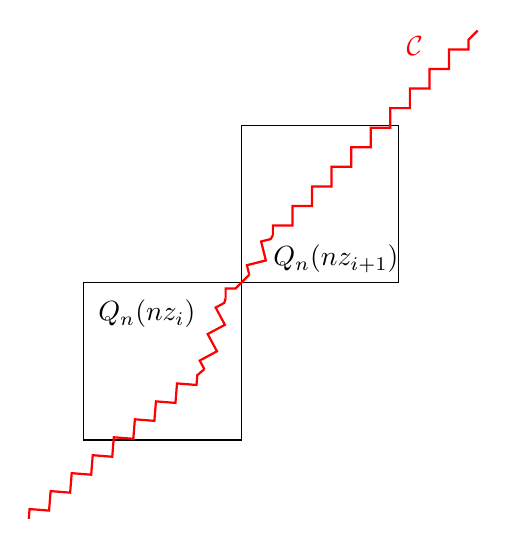
\begin{tikzpicture}
\draw (0,0) rectangle (2,2) ;
\draw (2,2) rectangle (4,4) ;
%\draw[red, thick, dashed] (-1,-1) .. controls (1.53,0.9) and (2,2)  .. (4,5);
\draw[red, thick, snake=zigzag] (-0.7,-1) -- (1.53,0.9) ;
\draw[red, thick, snake=zigzag] (1.53,0.9) -- (1.8,1.8) ;
\draw[red, thick, snake=zigzag] (1.8,1.8) -- (2,2) ;
\draw[red, thick] (2,2) -- (2.1,2.1) ;
\draw[red, thick, snake=zigzag] (2.1,2.1) -- (2.4,2.6) ;
\draw[red, thick, snake=zigzag] (2.4,2.6) -- (5,5.2) ;
\node[] at (0.8,1.6) {$Q_n(nz_i)$};
\node[] at (3.2,2.3) {$Q_n(nz_{i+1})$};
\node[text=red] at (4.2,5) {$\mathcal{C}$};
\end{tikzpicture}
\caption{Two consecutive $n$-bad sites have to share a common side}
\label{fig:connected-n-bad}
\end{figure}

Hence we get a contradiction, and so any two consecutive squares $Q_n(nz_i)$ and $Q_n(nz_{i+1})$ must share a common side. As a matter of fact, $\lbrace z_i, i \geq 1 \rbrace$ is a connected path in $\mathbb{Z}^2$  and we have therefore found an infinite path of $n$-bad sites. Hence, the process of $n$-bad sites percolates. 
\end{Proof}
By Lemma~\ref{Claim1.subcritical}, it suffices to prove that the process of $n$-bad sites does not percolate if $\lambda$ and $r$ are sufficiently small. This will be done via appealing to \cite[Theorem 0.0]{liggett_domination_1997}. \\
The conditions of \cite[Theorem 0.0]{liggett_domination_1997} are valid for so-called $k$-dependent random fields:
\begin{Definition}
Let $ \mathbf{X}=(X_s)_{s \in \mathbb{Z}^{d}}$ be a discrete random field. Let $k \geq 1$. Then $\mathbf{X}$ is said to be $k$-dependent if for all $p \geq 1$ and all $\psi = \lbrace s_{1}, \ldots s_{p} \rbrace \subset \mathbb{Z}^{d}$ finite with the property that $\forall i \neq j, \lVert s_{i} - s_{j} \rVert_{\infty} > k $, the random variables $(X_{s_{i}})_{1 \leq i \leq p}$ are independent.
\end{Definition}
%shall we keep d=2 there? 

As we shall see thereafter, the process of $n$-bad sites previously defined is $3$-dependent:

\begin{Lemma}
\label{Claim2.subcritical}
For $z \in \mathbb{Z}^{2}$, set $\zeta_{z} \coloneqq \mathbbm{1}\lbrace z \, \text{is $n$-bad} \rbrace$. Then $(\zeta_{z})_{z \in \mathbb{Z}^{2}}$ is a $3$-dependent random field.
\end{Lemma}
\begin{Proof}
As a starting point, note that $\forall z \in \mathbb{Z}^{2}, \zeta_{z} = 1 - \mathbbm{1} \lbrace z \, \text{is $n$-good} \rbrace$. It is therefore equivalent to prove that the process of $n$-good sites is $3$-dependent. \\
For $z \in \mathbb{Z}^{2}$, set $\xi_{z} = \mathbbm{1} \lbrace z \, \text{is $n$-good} \rbrace$. Let $\psi = \lbrace z_{1}, \ldots z_{p} \rbrace \subset \mathbb{Z}^{2}$ be such that $\forall i \neq j, \lVert z_i - z_j \rVert_{\infty} > 3$.
We want to show that the random variables $(\xi_{z_i})_{1\leq i \leq p}$ are independent. Since we are dealing with indicator functions, this is equivalent to showing that: 
$$\mathbb{E}\left(\prod_{i=1}^{p} \xi_{z_i} \right) = \prod_{i=1}^{p} \mathbb{E}(\xi_{z_i})$$
%Elie a fait une remarque là-dessus mais je ne suis pas sur d'avoir compris : c'est bien les variables aléatoires xi_z_i dont on veut montrer qu'elles sont indépendantes, ce qui équivaut à montrer que les événements incriminés sont indépendants, et donc in fine que l'espérance du produit est le produit des espérances ?
Now, we have:

\begin{align}
  \nonumber \mathbb{E}\left(\prod_{i=1}^{p} \xi_{z_i} \right) &= \mathbb{E}\left[\mathbb{E}\left(\prod_{i=1}^{p} \xi_{z_i} \Bigg\vert \Lambda \right)\right] \\ \label{eq2} &= \mathbb{E}\Bigg[\mathbb{E}\Bigg(\prod_{i=1}^{p}\mathbbm{1}\lbrace R(Q_n(nz_i)) < n \rbrace \prod_{i=1}^{p} \mathbbm{1} \lbrace \forall \, e \in E, \, s_{z_i,e} \, \text{is closed} \rbrace  \Bigg\vert \Lambda \Bigg) \Bigg] \\  &= \label{eq3}  \mathbb{E}\Bigg[\prod_{i=1}^{p} \mathbbm{1} \lbrace R(Q_n(nz_i) <n \rbrace \mathbb{E}\Bigg( \prod_{i=1}^{p} \mathbbm{1} \lbrace \forall \, e \in E, \, s_{z_i,e} \, \text{is closed} \rbrace  \Bigg\vert \Lambda \Bigg) \Bigg],
\end{align}
where we have used $\Lambda$-measurability of the random variables $\lbrace R_x \rbrace_{x \in \mathbb{R}^2}$ in~\eqref{eq3}. \\

For $1 \leq i \leq p$, set $A_{z_i} \coloneqq \lbrace \forall \, e \in E, \, s_{z_i,e} \, \text{is closed} \rbrace$. According to Definition~\ref{Def.open/closed/subcritical}, for a given $1 \leq i \leq p$, the event $A_{z_i}$ only depends on the configuration of the random measure $\Lambda$ and of the Cox process $X^{\lambda}$ inside the square $Q_n(nz_i)$. Therefore, given $\Lambda$, the events $\lbrace A_{z_i}  : 1 \leq i \leq p \rbrace$ only depend on $X^{\lambda} \cap Q_n(nz_i)$, $1 \leq i \leq p$. Since we have $\forall i \neq j, \lVert z_i - z_j \rVert_{\infty} > 3$, then the squares $Q_n(nz_i)$ are disjoint. Moreover, given $\Lambda$, $X^{\lambda}$ has the distribution of a Poisson Point Process. Thus, by Poisson independence property, the events $(A_{z_i})_{1 \leq i \leq p}$ are conditionally independent given $\Lambda$. Hence~\eqref{eq3} yields:
\begin{align}
 \label{eq4} \mathbb{E}\left(\prod_{i=1}^{p} \xi_{z_i} \right) &= \mathbb{E}\Bigg[\prod_{i=1}^{p} \mathbbm{1} \lbrace R(Q_n(nz_i) <n \rbrace \prod_{i=1}^{p} \mathbb{E}\Bigg(  \mathbbm{1} \lbrace \forall \, e \in E, \, s_{z_i,e} \, \text{is closed} \rbrace  \Bigg\vert \Lambda \Bigg) \Bigg] 
\end{align}
Set $f(\Lambda_{Q_n(x)}) \coloneqq \mathbb{E}\Bigg(  \mathbbm{1} \lbrace \forall \, e \in E, \, s_{x,e} \, \text{is closed} \rbrace  \Bigg\vert \Lambda \Bigg)$. Then $f$ is a deterministic, bounded and measurable function of $\Lambda_{Q_n(x)}$. Moreover,
%we are left with:
%\begin{align}
    %\mathbb{E}\left(\prod_{i=1}^{p} \xi_{z_i} \right) &= \mathbb{E}\left( \prod_{i=1}^{p} f(\Lambda_{Q_n(nz_i)}) \mathbbm{1}\lbrace R(Q_n(nz_i)) <n \rbrace \right) \label{eq5}
%\end{align}
the set $\varphi \coloneqq \lbrace nz_1,\ldots,nz_p \rbrace \subset \mathbb{R}^{d}$ is finite and satisfies: $$\forall i \neq j, \lVert nz_i - nz_j \rVert_{\infty} > 3n$$ Since the infinite norm is always upper bounded by the Euclidean norm, we have $\forall i \neq j, \lVert nz_i - nz_j \rVert_{2} > 3n $, and so $\varphi$ satisfies:
$$\forall x \in \varphi, \, \text{dist}(x, \varphi \setminus \lbrace x \rbrace) > 3n$$
Hence, by condition (3) in the definition of stabilization (Definition~\ref{Def.stabilizing}), the random variables appearing in the right-hand side of~\eqref{eq4} are independent. This yields:

\begin{align}
    \nonumber \mathbb{E}\left(\prod_{i=1}^{p} \xi_{z_i} \right)  &= \mathbb{E}\left( \prod_{i=1}^{p} f(\Lambda_{Q_n(nz_i)}) \mathbbm{1}\lbrace R(Q_n(nz_i)) <n \rbrace \right) \\ \label{eq5} &= \prod_{i=1}^{p} \mathbb{E}\left( f(\Lambda_{Q_n(nz_i)})\mathbbm{1}\lbrace R(Q_n(nz_i)) <n \rbrace \right) \\\nonumber &= \prod_{i=1}^{p} \mathbb{E}\left[  \mathbb{E}\Bigg(  \mathbbm{1} \lbrace \forall \, e \in E, \, s_{z_i,e} \, \text{is closed} \rbrace  \Bigg\vert \Lambda \Bigg) \mathbbm{1}\lbrace R(Q_n(nz_i)) <n \rbrace \right] \nonumber \\ &= \prod_{i=1}^{p} \mathbb{E}\left[  \mathbb{E}\Bigg(  \mathbbm{1} \lbrace \forall \, e \in E, \, s_{z_i,e} \, \text{is closed} \rbrace \mathbbm{1}\lbrace R(Q_n(nz_i)) <n \rbrace  \Bigg\vert \Lambda \Bigg)   \right]  \label{eq6}  \\ \nonumber &= \prod_{i=1}^{p} \mathbb{E}\left[   \mathbbm{1} \lbrace \forall \, e \in E, \, s_{z_i,e} \, \text{is closed} \rbrace \mathbbm{1}\lbrace R(Q_n(nz_i)) <n \rbrace \right] \\ \nonumber &\eqqcolon \prod_{i=1}^{p} \mathbb{E}(\xi_{z_i}), 
\end{align}
where we have used the aforementioned independence property in~\eqref{eq5} and $\Lambda$-measurability of the $R$'s in~\eqref{eq6}. This concludes the proof of the lemma.
\end{Proof}
Now that we have proven that the process of $n$-bad sites is $3$-dependent, in order to apply \cite[Theorem 0.0]{liggett_domination_1997}, it remains to prove that the probability for a site $z \in \mathbb{Z}^{d}$ to be $n$-bad is sufficiently small when $\lambda$ and $r$ are chosen sufficiently small. Equivalently, as has been done in \cite{hirsch2018continuum}, we need to prove the following:
\begin{equation*}
    \limsup_{n \uparrow \infty}\limsup_{r \downarrow 0}\limsup_{\lambda \downarrow 0} \mathbb{P}(z \, \text{is $n$-bad}) = 0
\end{equation*}
By stationarity, it suffices to prove that: 
\begin{equation*}
\limsup_{n \uparrow \infty}\limsup_{r \downarrow 0}\limsup_{\lambda \downarrow 0} \mathbb{P}(0 \, \text{is $n$-bad}) = 0
\end{equation*}
Now, note that we have:
\begin{align*}
    \mathbb{P}(0 \, \text{is $n$-bad}) &= \mathbb{P}\Big(\lbrace R(Q_n) \geq n \rbrace \cup \lbrace \exists \, e \in E, \, e \cap Q_n \, \text{is open} \rbrace \Big) \\ & \leq \mathbb{P}\left( R(Q_n) \geq n \right) + \mathbb{P}\left(  \exists \, e \in E, \, e \cap Q_n \, \text{is open} \right)
\end{align*}
On the one hand, we note that the quantity $R(Q_n)$ does not depend on $\lambda$ and $r$ and by Definition~\ref{Def.stabilizing}, we have $\displaystyle \lim_{n \uparrow \infty} \mathbb{P}(R(Q_n) \geq n)  = 0$, thus yielding: 
\begin{equation}
\label{eqsemifinalsubcritical}
  \limsup_{n \uparrow \infty} \limsup_{r \downarrow 0} \limsup_{\lambda \downarrow 0} \mathbb{P}(R(Q_n) \geq n)=0
\end{equation}
Therefore, it remains to deal with the quantity $\mathbb{P}\left(  \exists \, e \in E, \, e \cap Q_n \, \text{is open} \right)$. We have:
\begin{align}
    \nonumber \mathbb{P}\left(\exists \, e \in E, \, e \cap Q_n \, \text{is open} \right) &= 1 - \mathbb{P}\left(  \forall \, e \in E, \, e \cap Q_n \, \text{is closed} \right) \\ \nonumber &= 1 - \mathbb{E}\left( \prod_{e \in E \, : \, e \cap Q_n \neq \emptyset} \mathbbm{1}\lbrace \text{$e \cap Q_n$ is closed} \rbrace \right) \\ \nonumber &= 1 - \mathbb{E}\left[\mathbb{E}\left( \prod_{e \in E \, : e \cap Q_n \neq \emptyset} \mathbbm{1}\lbrace \text{$e \cap Q_n$ is closed} \rbrace  \Bigg\vert \Lambda \right) \right] 
\end{align}
For $e \in E$, denote:
\begin{gather*}
    s_e \coloneqq e \cap Q_n \\ A_e \coloneqq \lbrace \exists \, c \subset s_e, \, \text{$c$ topologically closed}, \vert c \vert = r, X^{\lambda}(c) = 0 \rbrace
\end{gather*}
We have: $\mathbbm{1}\lbrace \text{$s_e$ is closed} \rbrace = \mathbbm{1}\lbrace \vert s_e \vert > r \rbrace \mathbbm{1}\lbrace A_e \rbrace $. Thus:

\begin{align}
     \nonumber \mathbb{P}\left(\exists \, e \in E, \, e \cap Q_n \, \text{is open} \right) &= 1 - \mathbb{E}\left[\mathbb{E}\left( \prod_{e \in E \, : s_e \neq \emptyset} \mathbbm{1}\lbrace \vert s_e \vert > r \rbrace \mathbbm{1}\lbrace A_e \rbrace  \Bigg\vert \Lambda \right) \right] \\ \nonumber &= 1 - \mathbb{E}\left[\prod_{e \in E : s_e \neq \emptyset} \mathbbm{1}\lbrace \vert s_e \vert > r \rbrace\mathbb{E}\left( \prod_{e \in E \, : s_e \neq \emptyset}  \mathbbm{1}\lbrace A_e \rbrace  \Bigg\vert \Lambda \right) \right],  \intertext{by $\Lambda$-measurability of the events $\lbrace \vert s_e > r \vert \rbrace$,\, $e \in E$.} \nonumber
\end{align}
Given $\Lambda$, $X^{\lambda}$ has the distribution of a Poisson point process with mean measure $\lambda \Lambda$ and $A_e$ only depends on $X^{\lambda} \cap e$ once $e$ is fixed. Therefore, given $\Lambda$, the events $\lbrace A_e \, : e \in E \rbrace$ depend on the number of Cox points on distinct edges and so, by the Poisson independence property, these events are conditionally independent given $\Lambda$. Thus: 

\begin{align}
     \nonumber \mathbb{P}\left(\exists \, e \in E, \, e \cap Q_n \, \text{is open} \right) &= 1 - \mathbb{E}\left[\prod_{e \in E : s_e \neq \emptyset} \mathbbm{1}\lbrace \vert s_e \vert > r \rbrace\mathbb{E}\left( \prod_{e \in E \, : s_e \neq \emptyset}  \mathbbm{1}\lbrace A_e \rbrace  \Bigg\vert \Lambda \right) \right] \\ \nonumber &= 1 - \mathbb{E}\left[\prod_{e \in E : s_e \neq \emptyset} \mathbbm{1}\lbrace \vert s_e \vert > r \rbrace \prod_{e \in E \, : s_e \neq \emptyset}\mathbb{E}\left(   \mathbbm{1}\lbrace A_e \rbrace  \vert \Lambda \right) \right] \\ \label{eq7} &= 1 - \mathbb{E}\left[\prod_{e \in E : s_e \neq \emptyset} \mathbbm{1}\lbrace \vert s_e \vert > r \rbrace \prod_{e \in E \, : s_e \neq \emptyset}\mathbb{P}\left( A_e  \vert \Lambda \right) \right] 
\end{align}
For all $e \in E$ such that $s_e \neq \emptyset$, we have that $0 \leq \mathbb{P}(A_e \vert \Lambda) \leq 1$, and moreover the event $A_e$ is increasing in $\lambda$ with $\displaystyle \lim_{\lambda \downarrow 0} \mathbbm{1}\lbrace A_e \rbrace = 1 \: \text{a.s.}$. So, by monotone convergence, we have that for all $e \in E$ such that $s_e \neq \emptyset$, $\displaystyle \lim_{\lambda \downarrow 0} \mathbb{P}(A_e \vert \Lambda) = 1 \: \text{a.s.}$. As a matter of fact:
\begin{equation*}
    \limsup_{\lambda \downarrow 0} \prod_{e \in E : s_e \neq \emptyset} \mathbbm{1}\lbrace \vert s_e \vert > r \rbrace \prod_{e \in E \, : s_e \neq \emptyset}\mathbb{P}\left(    A_e  \vert \Lambda \right) = \prod_{e \in E : s_e \neq \emptyset} \mathbbm{1}\lbrace \vert s_e \vert > r \rbrace \quad \text{a.s.}
\end{equation*}
Noting that $\displaystyle \Bigg\lvert \prod_{e \in E : s_e \neq \emptyset} \mathbbm{1}\lbrace \vert s_e \vert > r \rbrace \prod_{e \in E \, : s_e \neq \emptyset}\mathbb{P}\left(    A_e  \vert \Lambda \right) \Bigg\rvert \leq 1$, we can apply dominated convergence in~\eqref{eq7}, we get:
\begin{align}
   \nonumber  \limsup_{\lambda \downarrow 0} \mathbb{P}\left(\exists \, e \in E, \, e \cap Q_n \, \text{is open} \right) &= 1 - \mathbb{E}\left(\prod_{e \in E : s_e \neq \emptyset} \mathbbm{1}\lbrace \vert s_e \vert > r \rbrace \right) \\ \label{eq8} &= \mathbb{P}(\exists \, e \in E, \, 0 < \vert e \cap Q_n \vert \leq r)
   %1 - \mathbb{E}\left(\prod_{e \in E} \mathbbm{1}\lbrace \vert e \cap Q_n \vert > r \rbrace \mathbbm{1} \lbrace e \cap Q_n \neq \emptyset \rbrace \right)
\end{align}
Note that for any fixed $\omega \in \Omega$, the event $\lbrace \exists \, e \in E, \, 0 < \vert e \cap Q_n \vert \leq r \rbrace$ is decreasing in $r$. Therefore, again by monotone convergence, we have for all $e \in E$:
\begin{align*}
\lim_{r \downarrow 0} \mathbb{P}(\exists \, e \in E, \, 0 < \vert e \cap Q_n \vert \leq r) &= 0
%\mathbbm{1}\lbrace \vert e \cap Q_n \vert > r \rbrace \mathbbm{1}\lbrace e \cap Q_n \neq \emptyset \rbrace 
%&= \mathbbm{1}\lbrace \vert e \cap Q_n \vert > 0 \rbrace \mathbbm{1}\lbrace e \cap Q_n \neq \emptyset \rbrace \quad \text{a.s.} \\ &= \mathbbm{1}\lbrace e \cap Q_n \neq \emptyset \rbrace \quad \text{a.s.}
\end{align*} 
Hence $\displaystyle \limsup_{r \downarrow 0} \mathbb{P}(\exists \, e \in E, \, 0 < \vert e \cap Q_n \vert \leq r) = 0$. Combining this with~\eqref{eq8} yields:
\begin{equation}
\label{eq9}
   \limsup_{r \downarrow 0}\limsup_{\lambda \downarrow 0} \mathbb{P}\left(\exists \, e \in E, \, e \cap Q_n \, \text{is open} \right) = 0
   %=1-\mathbb{E}\left(\prod_{e \in E } \mathbbm{1}\lbrace e \cap Q_n \neq \emptyset \rbrace \right)
\end{equation}
%By monotone convergence, $\displaystyle \lim_{n \uparrow \infty}\mathbbm{1}\lbrace e \cap Q_n \neq \emptyset \rbrace = 1 \quad \text{a.s.}$ for all $e \in E$. Therefore, by dominated convergence in~\eqref{eq9}, we obtain:
Hence, we obtain:
\begin{equation}
    \label{eq10}
    \limsup_{n \uparrow \infty}\limsup_{r \downarrow 0}\limsup_{\lambda \downarrow 0} \mathbb{P}\left(\exists \, e \in E, \, e \cap Q_n \, \text{is open} \right) = 1-1 = 0
\end{equation}
To conclude, we have: 
\begin{equation*}
    0 \leq \mathbb{P}(0 \, \text{is $n$-bad}) \leq \mathbb{P}(R(Q_n) \geq n) + \mathbb{P}(\exists \, e \in E, \, e \cap Q_n \, \text{is open})
\end{equation*}
Using~\eqref{eqsemifinalsubcritical} and~\eqref{eq10}, we finally get:
\begin{equation*}
     \limsup_{n \uparrow \infty}\limsup_{r \downarrow 0}\limsup_{\lambda \downarrow 0} \mathbb{P}(0 \, \text{is $n$-bad}) =0
\end{equation*}
Hence, by \cite[Theorem 0.0]{liggett_domination_1997}, the process of $n$-bad sites is stochastically dominated from above by a sub-critical Bernoulli process when $\lambda$ and $r$ are sufficiently small. In particular, the process of $n$-bad sites cannot percolate when $\lambda$ and $r$ are sufficiently small. In other words, there exists $r_0 >0$ such that $\lambda_c(r) > 0$. This concludes the proof of Theorem~\ref{Thm.subcritical}. \qed

\subsection{Proof of Corollary~\ref{Coroll.subcritical}}\mbox{}\\
Let $r_0$ be defined as in Theorem~\ref{Thm.subcritical}. Let $r \leq r_0$ and $p \in \left( p^{*},A \right]$. For fixed $\lambda > 0$, there are obviously fewer possible connections in the connectivity graph $\mathcal{G}_{p,\lambda,r}$ than in $\mathcal{G}_{1,\lambda,r}$. In other words, the vertex-set (resp. edge-set) of $\mathcal{G}_{p,\lambda,r}$ is a subset of the vertex-set (resp. edge-set) of $\mathcal{G}_{1, \lambda,r}$. Thus we have:
\begin{equation*}
    \mathcal{G}_{p,\lambda,r} \, \text{percolates} \,  \Rightarrow \mathcal{G}_{1,\lambda,r} \, \text{percolates}
\end{equation*}
Therefore:
\begin{equation*}
    \inf \lbrace \lambda > 0 : \, \mathbb{P}(\mathcal{G}_{p,\lambda,r} \; \text{percolates}) > 0 \rbrace >   \underbrace{\inf \lbrace \lambda > 0 : \, \mathbb{P}(\mathcal{G}_{1,\lambda,r} \; \text{percolates}) > 0 \rbrace}_{ \eqqcolon \lambda_c(r)}
\end{equation*}
By Theorem~\ref{Thm.subcritical}, we have that $\lambda_c(r) > 0$ whenever $r \leq r_0$. This concludes the proof of Corollary~\ref{Coroll.subcritical}. \qed

\subsection{Proof of Theorem~\ref{Thm.supercritical}}\mbox{}\\
As in the proof of Theorem~\ref{Thm.subcritical}, we will use a renormalization argument to prove that $\mathcal{G}_{p,\lambda,r}$ percolates if $\lambda$ and $p \in \left(p^{*},1\right]$ are chosen sufficiently large. \\
To this end, let us first define a discrete model in such a way that percolation of the discrete model will imply percolation of the continuum one. For $n \geq 1$, say a site $z \in \mathbb{Z}^{2}$ is $n$-good if the following conditions are satisfied:
\begin{enumerate}
\item $R(Q_{6n}(nz)) < n/2$ %3n/2 should be sufficient, double check if you need the stronger assumption n/2
\item $E \cap Q_n(nz) \neq \emptyset$, i.e. the square $Q_n(nz)$ contains a \emph{full} street segment (not just a subset of a street segment)
\item There exists $e \in E \cap Q_n(nz)$ such that $e$ is open, in the sense of Definition~\ref{Def.open/closed/subcritical}. In other words, there exists an open edge which is fully included in the square $Q_n(nz)$.
\item Every two open edges $e,e' \in E \cap Q_{3n}(nz)$ are connected by a path in $\mathcal{G}_{1,\lambda,r}\cap Q_{6n}(nz)$, i.e. $e$ and $e'$ are connected by a path of the connectivity graph staying inside of the larger square $Q_{6n}(nz)$ if all crossroads are open.
\item $Y(Q_{6n}(nz)) = \#(V \cap Q_{6n}(nz))$, i.e. all crossroads in $Q_{6n}(nz)$ are open, in the sense of Definition~\ref{Def.open/crossroad}.
\end{enumerate}
As in the proof of Theorem~\ref{Thm.subcritical}, for $n \geq 1$, say a site $z \in \mathbb{Z}^{2}$ is $n$-bad if it is not $n$-good. \\

The $n$-good sites have been defined so as to satisfy the following:
\begin{Lemma}
\label{Claim1.supercritical}
Percolation of the process of $n$-good sites implies percolation of the connectivity graph $\mathcal{G}_{p,\lambda,r}$.
\end{Lemma}
\begin{Proof}
Let $\mathcal{C}$ be an infinite connected component of $n$-good sites. Consider a finite path $\lbrace z_0, \ldots, z_q \rbrace \subset \mathcal{C}$ of $n$-good sites $(q \geq 1)$. Then, by condition $(2)$ in the definition of $n$-goodness, we can find an open edge $e_j \in E \cap Q_n(nz_j)$, for each $0 \leq j \leq q$. Let $0 \leq j \leq q-1$. Then $z_j = (a,b)$ for some $a \in \mathbb{Z}$ and $b \in \mathbb{Z}$. Since $\mathcal{C}$ is connected in $\mathbb{Z}^{2}$, we have $z_{j+1} \in \lbrace (a \pm 1, b), (a, b \pm 1) \rbrace$. By symmetry, we can assume $z_{j+1} = (a+1,b)$. Thus:
\begin{gather*}
Q_n(nz_j) = \left[na-n/2,na+n/2\right] \times \left[nb-n/2,nb+n/2\right]\\ Q_n(nz_{j+1}) = \left[na+n/2,na+3n/2\right] \times \left[nb-n/2,nb+n/2\right] \\
Q_{3n}(nz_j) = \left[na-3n/2,na+3n/2\right] \times \left[nb-3n/2,nb+3n/2\right] \\
Q_{6n}(nz_j) = \left[na-3n,na+3n\right] \times \left[nb-3n,nb+3n\right]
\end{gather*}
Therefore, we have $Q_{n}(nz_{j+1}) \subset Q_{3n}(nz_j)$ and so $e_{j+1} \in E \cap Q_{n}(nz_{j+1})$ implies $e_{j+1} \in E \cap Q_{3n}(nz_j)$. Since we also have $e_{j} \in E \cap Q_{n}(nz_j) \subset  E \cap Q_{3n}(nz_j)$ and that $e_j$ and $e_{j+1}$ are both open, by condition (4) in the definition of,$n$-goodness, $e_j$ and $e_{j+1}$ are connected by a path $\mathcal{L}$ in $\mathcal{G}_{1,\lambda,r} \cap Q_{6n}(nz_j)$. But since $z_j$ is an $n$-good site, by condition (5) in the definition of $n$-goodness, all crossroads inside of $Q_{6n}(nz_j)$ are open. Therefore, the path $\mathcal{L}$ also connects $e_j$ and $e_{j+1}$ in $\mathcal{G}_{p,\lambda,r} \cap Q_{6n}(nz_j)$. Iterating this process gives rise to an infinite connected component in $\mathcal{G}_{p,\lambda,r}$. This concludes the proof of Lemma~\ref{Claim1.supercritical}.
\end{Proof}
As a matter of fact, proving Theorem~\ref{Thm.supercritical} amounts to proving that the process of $n$-good sites percolates for sufficiently large $\lambda$ and $p$. \\
As has been done in the proof of Theorem~\ref{Thm.subcritical}, we will stochastically dominate the process of $n$-good sites by a Bernoulli process via the means of \cite[Theorem 0.0]{liggett_domination_1997}. To check that the conditions of this theorem are satisfied, we will need to use a slightly modified version of $n$-goodness more adapted to the use of the aforementioned theorem, as follows: \\

For $n \geq 1$, say a site $z \in \mathbb{Z}^{2}$ is weakly-$n$-good if the following conditions are satisfied:
\begin{enumerate}
\item[$\widetilde{(1)}$] $R(Q_{6n}(nz)) < 6n$
\item[(2)]  $E \cap Q_n(nz) \neq \emptyset$, i.e. the square $Q_n(nz)$ contains a \emph{full} street segment (not just a subset of a street segment)
\item[(3)]  There exists $e \in E \cap Q_n(nz)$ such that $e$ is open, in the sense of Definition~\ref{Def.open/closed/subcritical}. In other words, there exists an open edge which is fully included in the square $Q_n(nz)$.
\item[(4)]  Every two open edges $e,e' \in E \cap Q_{3n}(nz)$ are connected by a path in $\mathcal{G}_{1,\lambda,r}\cap Q_{6n}(nz)$, i.e. $e$ and $e'$ are connected by a path of the connectivity graph staying inside of the larger square $Q_{6n}(nz)$ if all crossroads are open.
\item[(5)]  $Y(Q_{6n}(nz)) = \#(V \cap Q_{6n}(nz))$, i.e. all crossroads in $Q_{6n}(nz)$ are open, in the sense of Definition~\ref{Def.open/crossroad}.
\end{enumerate}
Note that the difference between $n$-goodness and weakly-$n$-goodness only lies in the first condition $(1) \; R(Q_{6n}(nz))<n/2$ being weakened into $\widetilde{(1)} \; R(Q_{6n}(nz))< 6n$. All other conditions remain unchanged. \\

Then the following is clear:
\begin{Lemma}
\label{Lemma1.almost}
$\forall \, z \in \mathbb{Z}^{2}$, $z$ is $n$-good $\Rightarrow \, z$ is weakly-$n$-good. Therefore, we have the following: $\forall \, z \in \mathbb{Z}^{2}, \: \mathbb{P}(\text{$z$ is $n$-good}) \leq \mathbb{P}(\text{$z$ is weakly-$n$-good})$
\end{Lemma} Moreover, since the condition (1) in the definition of $n$-goodness has not been used in the proof of Lemma~\ref{Claim1.supercritical}, the following is also clear:
\begin{Lemma}
\label{Lemma2.almost}
Percolation of the process of weakly-$n$-good sites implies percolation of the connectivity graph $\mathcal{G}_{p,\lambda,r}$.
\end{Lemma}
The reason why considering almost-$n$-good sites instead of $n$-good sites will turn out to be easier for our purposes is the following:
\begin{Lemma}
\label{Claim2.supercritical}
For $z \in \mathbb{Z}^{2}$, set $\xi_{z} \coloneqq \mathbbm{1}\lbrace z \, \text{is weakly-$n$-good} \rbrace$. Then $(\xi_{z})_{z \in \mathbb{Z}^{2}}$ is an $18$-dependent random field.
\end{Lemma}
\begin{Proof}
In the same way as in the proof of Lemma~\ref{Claim1.subcritical}, it suffices to prove that for all finite $\psi = \lbrace z_{1}, \ldots z_{p} \rbrace \subset \mathbb{Z}^{2}$ such that $\forall i \neq j, \lVert z_i - z_j \rVert_{\infty} > 18$, we have:
$$\mathbb{E}\left(\prod_{i=1}^{p} \xi_{z_i} \right) = \prod_{i=1}^{p} \mathbb{E}(\xi_{z_i})$$
Denote respectively by $\widetilde{(A_z)},(B_z),(C_z),(D_z),(F_z)$ the events $\widetilde{(1)},(2),(3),(4),(5)$ in the definition of weakly-$n$-goodness for $z \in \mathbb{Z}^{2}$. We thus have: 
$$\forall z \in \mathbb{Z}^{2}, \, \xi_{z} = \mathbbm{1}\lbrace \widetilde{(A_z)} \rbrace \mathbbm{1}\lbrace (B_z) \rbrace \mathbbm{1}\lbrace (C_z) \rbrace \mathbbm{1}\lbrace (D_z) \rbrace \mathbbm{1}\lbrace (F_z) \rbrace$$

Note first that whenever $z \in \mathbb{Z}^{2}$, the indicators $\mathbbm{1} \lbrace \widetilde{(A_z)} \rbrace$ and $\mathbbm{1} \lbrace (B_z) \rbrace$ are $\Lambda$-measurable. Thus, we have :
\begin{align}
\nonumber \mathbb{E}\left(\prod_{i=1}^{p} \xi_{z_i} \right) &= \mathbb{E}\left[\mathbb{E}\left(\prod_{i=1}^{p} \xi_{z_i} \Bigg\vert \Lambda \right)\right] 
\\ \nonumber &= \mathbb{E}\left[\mathbb{E}\left(\prod_{i=1}^{p} \mathbbm{1}\lbrace \widetilde{(A_{z_i})} \rbrace \mathbbm{1}\lbrace (B_{z_i}) \rbrace \mathbbm{1}\lbrace (C_{z_i}) \rbrace \mathbbm{1}\lbrace (D_{z_i}) \rbrace \mathbbm{1}\lbrace (F_{z_i}) \rbrace \Bigg\vert \Lambda \right)\right] 
\\ \nonumber &= \mathbb{E}\left[\prod_{i=1}^{p} \mathbbm{1}\lbrace \widetilde{(A_{z_i})} \rbrace \mathbbm{1}\lbrace (B_{z_i})\rbrace\mathbb{E}\left(  \prod_{i=1}^{p}\mathbbm{1}\lbrace (C_{z_i}) \cap (D_{z_i}) \cap (F_{z_i})  \rbrace \Bigg\vert \Lambda \right)\right] 
\end{align}
Now, note that conditioned on $\Lambda$, for each $1 \leq i \leq p$, the event $ (C_{z_i}) \cap (D_{z_i}) \cap (F_{z_i}) $ only depends on the following:
\begin{itemize}
\item The configuration of $X^{\lambda}$ inside of the square $Q_{6n}(nz_i)$
\item The configuration of $Y$ inside of the square $Q_{6n}(nz_i)$
\end{itemize}
Since $\psi$ satisfies $\forall i \neq j, \lVert z_i - z_j \rVert_{\infty} > 18$, then we have $\forall i \neq j, \lVert nz_i - nz_j \rVert_{\infty} > 18n$. As a matter of fact, the squares $\lbrace Q_{6n}(nz_i)) \, : \, 1 \leq i \leq p\rbrace$ are disjoint, i.e. $$\forall i \neq j, Q_{6n}(nz_i) \cap Q_{6n}(nz_j) = \emptyset$$
As a matter of fact, the events $\lbrace (C_{z_i}) \cap (D_{z_i}) \cap (F_{z_i}) \, : \, 1 \leq i \leq p \rbrace$ depend on disjoint Borel sets. 
%so, by the independence property of Z
Now, conditioned on $\Lambda$, $X^{\lambda}$ has the distribution of a Poisson point process, $Y$ has the distribution of a Bernoulli point process and $X^{\lambda} \indep Y \, \vert \Lambda \,$. By the independence property for Poisson and Bernoulli point processes, we have that the events $ \lbrace (C_{z_i}) \cap (D_{z_i}) \cap (F_{z_i}) \, : \, 1 \leq i \leq p \rbrace$ are conditionally independent given $\Lambda$. Hence:
\begin{align}
\nonumber \mathbb{E}\left(\prod_{i=1}^{p} \xi_{z_i} \right)  &= \mathbb{E}\left[\prod_{i=1}^{p} \mathbbm{1}\lbrace \widetilde{(A_{z_i})} \rbrace \mathbbm{1}\lbrace (B_{z_i})\rbrace\mathbb{E}\left(  \prod_{i=1}^{p}\mathbbm{1}\lbrace (C_{z_i}) \cap (D_{z_i}) \cap (F_{z_i})  \rbrace \Bigg\vert \Lambda \right)\right] 
\\ \nonumber &=  \mathbb{E}\left[\prod_{i=1}^{p} \mathbbm{1}\lbrace \widetilde{(A_{z_i})} \rbrace \mathbbm{1}\lbrace (B_{z_i})\rbrace \prod_{i=1}^{p}\mathbb{E}\left(  \mathbbm{1}\lbrace (C_{z_i}) \cap (D_{z_i}) \cap (F_{z_i})  \rbrace \Bigg\vert \Lambda \right)\right] 
\end{align}
Again, by $\Lambda$-measurability of the events $ \lbrace (B_{z_i}) \, : \, 1 \leq i \leq p \rbrace$, we can put the indicators $\mathbbm{1} \lbrace (B_{z_i}) \rbrace$ back into the conditional expectation given $\Lambda$, so as to get:
\begin{align}
\nonumber \mathbb{E}\left(\prod_{i=1}^{p} \xi_{z_i} \right)  &=  \mathbb{E}\left[\prod_{i=1}^{p} \mathbbm{1}\lbrace \widetilde{(A_{z_i})} \rbrace  \prod_{i=1}^{p}\mathbb{E}\left( \mathbbm{1}\lbrace (B_{z_i})\rbrace \mathbbm{1}\lbrace (C_{z_i}) \cap (D_{z_i}) \cap (F_{z_i})  \rbrace \Bigg\vert \Lambda \right)\right] 
\\ \nonumber &= \mathbb{E}\left[\prod_{i=1}^{p} \mathbbm{1}\lbrace \widetilde{(A_{z_i})} \rbrace  \prod_{i=1}^{p}\mathbb{E}\left( \mathbbm{1}\lbrace (B_{z_i}) \cap (C_{z_i}) \cap (D_{z_i}) \cap (F_{z_i})  \rbrace \Bigg\vert \Lambda \right)\right] 
\end{align}
Now, setting $f(\Lambda_{Q_{6n}(x)}) \coloneqq \mathbb{E}\left(\mathbbm{1}\lbrace (B_{x}) \cap (C_{x}) \cap (D_{x}) \cap (F_{x})  \rbrace \,  \vert \, \Lambda \right)$, a bounded measurable deterministic function of $\Lambda_{Q_{6n}(x)}$, we are left with:
\begin{align}
\nonumber \mathbb{E}\left(\prod_{i=1}^{p} \xi_{z_i} \right)  &=  \mathbb{E}\left[\prod_{i=1}^{p} \mathbbm{1}\lbrace \widetilde{(A_{z_i})} \rbrace  \prod_{i=1}^{p}\mathbb{E}\left( \mathbbm{1}\lbrace (B_{z_i})\rbrace \mathbbm{1}\lbrace (C_{z_i}) \cap (D_{z_i}) \cap (F_{z_i})  \rbrace \Bigg\vert \Lambda \right)\right] 
\\ \label{eq11} &= \mathbb{E}\left[\prod_{i=1}^{p} \mathbbm{1}\lbrace R(Q_{6n}(nz_i) < 6n \rbrace  f(\Lambda_{Q_{6n}(nz_i)})\right] 
\end{align}
Now, the set $\varphi \coloneqq \lbrace nz_1,\ldots,nz_p \rbrace \subset \mathbb{R}^{d}$ is finite and satisfies: $$\forall i \neq j, \lVert nz_i - nz_j \rVert_{\infty} > 18n $$ Since the infinite norm is always upper bounded by the Euclidean norm, we have $\forall i \neq j, \lVert nz_i - nz_j \rVert_{2} > 18n  $, and so $\varphi$ satisfies:
$$\forall x \in \varphi, \, \text{dist}(x, \varphi \setminus \lbrace x \rbrace) > 18n=3 \times 6n $$
We can therefore apply condition (3) in Definition~\ref{Def.stabilizing} (with $n$ replaced by $6n$) to get that the random variables appearing in the right-hand side of~\eqref{eq11} are independent. Hence:
\begin{align}
\label{eq12} \mathbb{E}\left(\prod_{i=1}^{p} \xi_{z_i} \right)  &= \prod_{i=1}^{p} \mathbb{E}\left[\mathbbm{1}\lbrace R(Q_{6n}(nz_i) < 6n \rbrace   f(\Lambda_{Q_{6n}(nz_i)})\right] 
\end{align}
Now, for each $1 \leq i \leq p$, note that:
\begin{gather*}
 \mathbb{E}\left[\mathbbm{1}\lbrace R(Q_{6n}(nz_i) < 6n \rbrace   f(\Lambda_{Q_{6n}(nz_i)})\right] 
\\  = \mathbb{E}\left[\mathbbm{1}\lbrace R(Q_{6n}(nz_i) < 6n \rbrace  \mathbb{E}\left(\mathbbm{1}\lbrace (B_{z_i}) \cap (C_{z_i}) \cap (D_{z_i}) \cap (F_{z_i})  \rbrace \,  \vert \, \Lambda \right)  \right]
\\ = \mathbb{E}\left[ \mathbb{E}\left(\mathbbm{1}\lbrace R(Q_{6n}(nz_i) < 6n \rbrace \mathbbm{1}\lbrace (B_{z_i}) \rbrace \mathbbm{1} \lbrace (C_{z_i}) \rbrace \mathbbm{1} \lbrace (D_{z_i}) \rbrace \mathbbm{1} \lbrace (F_{z_i})  \rbrace \,  \Bigg\vert \, \Lambda \right)  \right],
\\ \intertext{using $\Lambda$-measurability of $\mathbbm{1}\lbrace R(Q_{6n}(nz_i) < 6n \rbrace$}
\\ =  \mathbb{E}\left(\mathbbm{1}\lbrace R(Q_{6n}(nz_i) < 6n \rbrace \mathbbm{1}\lbrace (B_{z_i}) \rbrace \mathbbm{1} \lbrace (C_{z_i}) \rbrace \mathbbm{1} \lbrace (D_{z_i}) \rbrace \mathbbm{1} \lbrace (F_{z_i})  \rbrace \right)
\\ =  \mathbb{E}\left(\mathbbm{1}\lbrace (A_{z_i}) \rbrace \mathbbm{1}\lbrace (B_{z_i}) \rbrace \mathbbm{1} \lbrace (C_{z_i}) \rbrace \mathbbm{1} \lbrace (D_{z_i}) \rbrace \mathbbm{1} \lbrace (F_{z_i})  \rbrace \right) 
\\ \eqqcolon \mathbb{E}(\xi_{z_i})
\end{gather*}
Thus,~\eqref{eq12} yields:
\begin{equation*}
 \mathbb{E}\left(\prod_{i=1}^{p} \xi_{z_i} \right) = \prod_{i=1}^{p} \mathbb{E}(\xi_{z_i}),
\end{equation*}
as needed. This concludes the proof of Lemma~\ref{Claim2.supercritical}.
\end{Proof}
Our intention is to apply \cite[Theorem 0.0]{liggett_domination_1997} and stochastically dominate from below the process of weakly-$n$-good sites by a supercritical Bernoulli process. Since percolation of the weakly-$n$-good sites implies percolation of $\mathcal{G}_{p,\lambda,r}$, we will be done. \\

Now that we have proven that  the process of weakly-$n$-good sites is $18$-dependent, to apply \cite[Theorem 0.0]{liggett_domination_1997}, it remains to prove that the probability $z \in \mathbb{Z}^{d}$ to be weakly-$n$-good is arbitrarily large when $\lambda$ and $p$ are sufficiently large. Equivalently, as has been done in the proof of Theorem~\ref{Thm.subcritical}, we need to prove the following:
\begin{equation*}
    \limsup_{n \uparrow \infty}\limsup_{\lambda \uparrow \infty}\limsup_{p \uparrow 1} \mathbb{P}(z \, \text{is weakly-$n$-good}) = 1
\end{equation*}
By stationarity, it suffices to prove that: 
\begin{equation*}
\limsup_{n \uparrow \infty}\limsup_{\lambda \uparrow \infty}\limsup_{p \uparrow 1} \mathbb{P}(0 \, \text{is weakly-$n$-good}) = 1
\end{equation*}
Since $ \mathbb{P}(\text{$0$ is $n$-good}) \leq \mathbb{P}(\text{$0$ is weakly-$n$-good})$, it suffices to prove that:
\begin{equation*}
\limsup_{n \uparrow \infty}\limsup_{\lambda \uparrow \infty}\limsup_{p \uparrow 1} \mathbb{P}(0 \, \text{is $n$-good}) = 1
\end{equation*}
Or, equivalently:
\begin{equation*}
\limsup_{n \uparrow \infty}\limsup_{\lambda \uparrow \infty}\limsup_{p \uparrow 1} \mathbb{P}(0 \, \text{is $n$-bad}) = 0
\end{equation*}
For $z \in \mathbb{Z}^{2}$, denote respectively by $(A_z),(B_z), (C_z), (D_z), (F_z)$ the events (1), (2), (3), (4), (5) in the definition of $n$-goodness. Denote by $(A),(B),(C),(D),(F)$ the former events for $z=0$. We have:
\begin{align*}
    \mathbb{P}(0 \, \text{is $n$-bad}) &= \mathbb{P}(A^c \cup B^c \cup C^c \cup D^c \cup F^c)
\\ &= \mathbb{P}(A^c) + \mathbb{P}(A \cap B^c) + \mathbb{P}(A \cap B \cap C^c) + \mathbb{P}(A \cap B \cap C \cap F^c) \\ & \quad + \mathbb{P}(A \cap B \cap C \cap F \cap D^c)
\end{align*}
First, partitioning the square $Q_{6n}$ into $12^2=144$ subsquares $(Q_i)_{1 \leq i \leq 144}$ of side length $n/2$, we get:
\begin{align}
    \nonumber \mathbb{P}(A^c) &= \mathbb{P}(R(Q_{6n}) \geq n/2)
    \\ \nonumber & \leq  \mathbb{P}\left(\bigcup_{i=1}^{144} \left\lbrace  R(Q_i) \geq n/2 \right\rbrace \right)
    \\ \nonumber &= 144 \; \mathbb{P}(R(Q_{n/2}) \geq n/2) \qquad \text{by stationarity of the $R$'s} 
\end{align}
Therefore, by condition (2) of Definition~\ref{Def.stabilizing}, we get: $\lim_{n \uparrow \infty} \mathbb{P}(A^c) = 0$. Noting that the event $A^c$ does not depend on $\lambda$ and $p$, the former yields:
\begin{equation}
    \label{eq13}
    \limsup_{n \uparrow \infty}\limsup_{\lambda \uparrow \infty}\limsup_{p \uparrow 1} \mathbb{P}(A^c) = \limsup_{n \uparrow \infty} \mathbb{P}(A^c)= \lim_{n \uparrow \infty} \mathbb{P}(A^c) = 0
\end{equation}
Moreover, we have: 
\begin{align*}
    \mathbb{P}(A \cap B^c) & \leq \mathbb{P}(B^c)
    \\ & \eqqcolon \mathbb{P}(E \cap Q_n = \emptyset)
\end{align*}
By monotone convergence, we therefore get:
\begin{equation*}
    \lim_{n \uparrow \infty}\mathbb{P}(E \cap Q_n = \emptyset) = \mathbb{P}(E \cap \mathbb{R}^{2} = \emptyset) = 0,
\end{equation*}
since $\lambda_S > 0$ and so the Poisson-Voronoi tessellation $S$ is non-empty. Therefore, we have $\lim_{n \uparrow \infty}\mathbb{P}(A \cap B^c) = 0$. Since the event $A \cap B^c$ only depends on $n$, we get:
\begin{equation}
    \label{eq14}
    \limsup_{n \uparrow \infty}\limsup_{\lambda \uparrow \infty}\limsup_{p \uparrow 1}\mathbb{P}(A \cap B^c) = \limsup_{n \uparrow \infty}\mathbb{P}(A \cap B^c)= \lim_{n \uparrow \infty}\mathbb{P}(A \cap B^c) = 0
\end{equation}
Let's now deal with the quantity $\mathbb{P}(A \cap B \cap C^c)$. We have:
\begin{align*}
    \mathbb{P}(A \cap B \cap C^c) &\leq \mathbb{P}(B \cap C^c)
    \\ &= \mathbb{P}(\lbrace E \cap Q_n \neq \emptyset \rbrace \cap \lbrace \forall \, e \in E \cap Q_n, e \, \text{is closed} \rbrace)
    \\ &= \mathbb{E}\left( \mathbbm{1}\lbrace E \cap Q_n \neq \emptyset \rbrace \prod_{e \in E \cap Q_n} \mathbbm{1} \lbrace e \, \text{is closed} \rbrace \right)
    \\ &= \mathbb{E}\left[\mathbb{E}\left(\mathbbm{1}\lbrace E \cap Q_n \neq \emptyset \rbrace \prod_{e \in E \cap Q_n} \mathbbm{1} \lbrace e \, \text{is closed} \rbrace \Bigg\vert \Lambda \right)\right]
\end{align*}
The event $\lbrace E \cap Q_n \rbrace$ is $\Lambda$-measurable, hence:
\begin{align}
\label{eq15}
    \mathbb{P}(A \cap B \cap C^c) &\leq \mathbb{E}\left[\mathbbm{1}\lbrace E \cap Q_n \neq \emptyset \rbrace\mathbb{E}\left( \prod_{e \in E \cap Q_n} \mathbbm{1} \lbrace e \, \text{is closed} \rbrace \Bigg\vert \Lambda \right)\right]
\end{align}
Now, we have:
\begin{gather*}
\mathbb{E}\left( \prod_{e \in E \cap Q_n} \mathbbm{1} \lbrace e \, \text{is closed} \rbrace \Bigg\vert \Lambda \right) \\
=\mathbb{E}\left( \prod_{e \in E \cap Q_n} \mathbbm{1} \lbrace \vert e \vert > r \rbrace \mathbbm{1} \lbrace \exists  \, c \subset s, \, \vert c \vert = r \; , \, c  \, \text{topologically closed} \,  ,  X^{\lambda}(c) = 0 \rbrace \Bigg\vert \Lambda \right)
\end{gather*}
For each $e \in E \cap Q_n$, denote:
$$I_e \coloneqq \lbrace \exists \, c \subset s, \; \text{such that} \, \vert c \vert = r \; \text{and} \; c  \; \text{topologically closed} \; \text{and} \,  X^{\lambda}(c) = 0 \rbrace$$
Since the event $\lbrace \vert e \vert > r \rbrace$ is $\Lambda$-measurable for each $e \in E \cap Q_n$, we get:
\begin{equation*}
\mathbb{E}\left( \prod_{e \in E \cap Q_n} \mathbbm{1} \lbrace e \, \text{is closed} \rbrace \Bigg\vert \Lambda \right) = \prod_{e \in E \cap Q_n} \mathbbm{1} \lbrace \vert e \vert > r \rbrace \mathbb{E}\left( \prod_{e \in E \cap Q_n}  \mathbbm{1} \lbrace I_e \rbrace \Bigg\vert \Lambda \right)
\end{equation*}
Conditioned on $\Lambda$, $X^{\lambda}$ has the distribution of a Poisson point process, and the events $\lbrace I_e : e \in E \cap Q_n \rbrace$ depend on the configuration of $X^{\lambda}$ distinct edges. Therefore, by the Poisson independence property, the events $\lbrace I_e : e \in E \cap Q_n \rbrace$ are conditionally independent given $\Lambda$. This yields:
\begin{align}
\nonumber \mathbb{E}\left( \prod_{e \in E \cap Q_n} \mathbbm{1} \lbrace e \, \text{is closed} \rbrace \Bigg\vert \Lambda \right) &= \prod_{e \in E \cap Q_n} \mathbbm{1} \lbrace \vert e \vert > r \rbrace \mathbb{E}\left( \prod_{e \in E \cap Q_n}  \mathbbm{1} \lbrace I_e \rbrace \Bigg\vert \Lambda \right)
\\ \nonumber  &= \prod_{e \in E \cap Q_n} \mathbbm{1} \lbrace \vert e \vert > r \rbrace \mathbb{E}\left(  \mathbbm{1} \lbrace I_e \rbrace \vert \Lambda \right)
\\ \nonumber &= \prod_{e \in E \cap Q_n} \mathbbm{1} \lbrace \vert e \vert > r \rbrace \mathbb{P}\left(   I_e  \vert \Lambda \right)
\\ \label{eq16} &= \prod_{e \in E \cap Q_n} \mathbbm{1} \lbrace \vert e \vert > r \rbrace \prod_{e \in E \cap Q_n}\mathbb{P}\left(   I_e  \vert \Lambda \right)
\end{align}
Since the support will be filled with Cox points as $\lambda \uparrow \infty$, it is clear by monotone convergence that $\displaystyle \forall e \in E \cap Q_n, \, \limsup_{\lambda \uparrow \infty} \mathbb{P}(I_e \vert \Lambda) = 0 \; \text{a.s.}$. Since the cardinal of $E \cap Q_n$ does not depend on $\lambda$ and since the events $\lbrace \vert e \vert > r \; : \; e \in E \cap Q_n \rbrace$ do not depend on $\lambda$ either, using monotone convergence in~\eqref{eq16}, we get:
\begin{align}
   \nonumber  \limsup_{\lambda \uparrow \infty} \mathbb{E}\left( \prod_{e \in E \cap Q_n} \mathbbm{1} \lbrace e \, \text{is closed} \rbrace \Bigg\vert \Lambda \right) &= \left(\prod_{e \in E \cap Q_n} \mathbbm{1} \lbrace \vert e \vert > r \rbrace \right) \mathbbm{1}\lbrace E \cap Q_n = \emptyset \rbrace \; \text{a.s.}
   \\ \label{eq17} &= \mathbbm{1} \lbrace E \cap Q_n = \emptyset \rbrace \; \text{a.s.},
\end{align}
where~\eqref{eq17} is obtained by distinguishing both cases $E \cap Q_n = \emptyset$ and $E \cap Q_n \neq \emptyset$. \\
Getting back to~\eqref{eq15} and applying dominated convergence on the right-hand side with the use of~\eqref{eq17}, we therefore get:
\begin{equation*}
  \limsup_{\lambda \uparrow \infty} \mathbb{P}(A \cap B \cap C^c) \leq \mathbb{E}\left[\mathbbm{1}\lbrace E \cap Q_n \neq \emptyset \rbrace \mathbbm{1} \lbrace E \cap Q_n = \emptyset \rbrace \right] = 0  
\end{equation*}
Hence $\limsup_{\lambda \uparrow \infty} \mathbb{P}(A \cap B \cap C^c) = 0$. Now, note that the event $A \cap B \cap C^c$ only depends on $n$ and $\lambda$. Therefore:
\begin{equation*}
   \limsup_{\lambda \uparrow \infty}\limsup_{p \uparrow 1} \mathbb{P}(A \cap B \cap C^c) = \limsup_{\lambda \uparrow \infty} \mathbb{P}(A \cap B \cap C^c) = 0
\end{equation*}
and so:
\begin{equation}
    \label{eq18}
    \limsup_{n \uparrow \infty}\limsup_{\lambda \uparrow \infty}\limsup_{p \uparrow 1} \mathbb{P}(A \cap B \cap C^c) = 0
\end{equation}
We now deal with the quantity $\mathbb{P}(A \cap B \cap C \cap F^c)$. We have: 
%is it 1-p^\#(V ...) or (1-p)^\#(V ...) : adapt in consequence!
\begin{align*}
    \mathbb{P}(A \cap B \cap C \cap F^c) &\leq \mathbb{P}(F^{c})
    \\ &= \mathbb{E}(\mathbbm{1}\lbrace F^c \rbrace)
    \\ &= \mathbb{E}(1-\mathbbm{1}\lbrace F \rbrace)
    \\ &= \mathbb{E}\left[1-\mathbb{E}(\mathbbm{1}\lbrace F \rbrace \vert \Lambda ) \right]
    \\ &= \mathbb{E}\left[1-\mathbb{E}\left( \prod_{v \in V \cap Q_{6n}} \mathbbm{1}\lbrace v \, \text{is open} \rbrace \Bigg\vert \Lambda \right)\right]
\end{align*}
By definition of $Y$, the random variables $(\mathbbm{1} \lbrace v \, \text{is open} \rbrace )_{v \in V}$ are conditionally independent given $\Lambda$, so we get:
\begin{align}
    \nonumber \mathbb{P}(A \cap B \cap C \cap F^c) &\leq \mathbb{E}\left[1-\prod_{v \in V \cap Q_{6n}}\mathbb{E}\left( \mathbbm{1}\lbrace v \, \text{is open} \rbrace \vert \Lambda \right)\right]
    \\ \nonumber &= \mathbb{E}\left[1-\prod_{v \in V \cap Q_{6n}}\mathbb{P}\left( v \, \text{is open} \vert \Lambda \right)\right]
    \\ \label{eq19} &= \mathbb{E}\left[1-p^{\#(V \cap Q_{6n})}\right], 
\end{align}
where the last line comes directly from the definition of $Y$. By monotone convergence, we have:
\begin{align*}
  \lim_{p \uparrow 1}1-p^{\#(V \cap Q_{6n})} &= 0 \; \text{a.s. for all finite } n \geq 0
  %\mathbbm{1}\lbrace \#(V \cap Q_{6n}) = \infty  \rbrace \; \text{a.s.}
  %\\ &= \mathbbm{1}\lbrace V \cap Q_{6n} = \emptyset \rbrace \; \text{a.s.}  
\end{align*}
Hence, using dominated convergence in the right-hand side of~\eqref{eq19}, we get:
\begin{align*}
\lim_{p \uparrow 1} \mathbb{P}(A \cap B \cap C \cap F^c) = 0 \; \text{for all finite } n \geq 0
%&\leq \mathbb{E}(\mathbbm{1}\lbrace V \cap Q_{6n} = \emptyset \rbrace)
%\\ &= \mathbb{P}(V \cap Q_{6n} = \emptyset)
\end{align*}
Hence $\limsup_{p \uparrow 1}1-p^{\#(V \cap Q_{6n})} = 0 \; \text{a.s. for all finite } n \geq 0$. \\
Note that the right-hand side of the former equality does not depend on $\lambda$. Therefore, we have: \begin{equation*}
    \limsup_{\lambda \uparrow \infty}\lim_{p \uparrow 1} \mathbb{P}(A \cap B \cap C \cap F^c) = 0 \; \text{for all finite } n \geq 0
    %\leq \limsup_{\lambda \uparrow \infty} \mathbb{P}(V \cap Q_{6n} = \emptyset) = \mathbb{P}(V \cap Q_{6n} = \emptyset)
\end{equation*}
And so:
%by monotone convergence:
\begin{align*}
%\limsup_{n \uparrow \infty}\limsup_{\lambda \uparrow \infty}\lim_{p \uparrow 1} \mathbb{P}(A \cap B \cap C \cap F^c) &= 
\lim_{n \uparrow \infty}\limsup_{\lambda \uparrow \infty}\lim_{p \uparrow 1} \mathbb{P}(A \cap B \cap C \cap F^c) &=0
%&\leq \limsup_{n \uparrow \infty} \mathbb{P}(V \cap Q_{6n} = \emptyset) \\ &= \lim_{n \uparrow \infty} \mathbb{P}(V \cap Q_{6n} = \emptyset)
%\\ &= \mathbb{P}(V \cap \mathbb{R}^{2} = \emptyset)
%\\ &= 0 \quad \text{since $\lambda_{S} > 0$, and so $V \neq \emptyset$}
\end{align*}
Therefore, we finally have:
\begin{equation}
    \label{eq20}
    \limsup_{n \uparrow \infty} \limsup_{\lambda \uparrow \infty} \limsup_{p \uparrow 1} \mathbb{P}(A \cap B \cap C \cap F^c)=0
    %=\lim_{n \uparrow \infty}\limsup_{\lambda \uparrow \infty}\lim_{p \uparrow 1} \mathbb{P}(A \cap B \cap C \cap F^c) = 0
\end{equation}
It finally remains to deal with the quantity $\mathbb{P}(A \cap B \cap C \cap F \cap D^{c})$. \\
First, note that only the events $A$ and $B$ only depend on $n$ and the underlying random support given by $\Lambda$, while the event $F$ only depends on $p$. The events $C$ and $D^c$ both depend on $\Lambda$, $n$ and $\lambda$. For fixed $n$ and $\lambda$, we first deal with the limit in $p$ as follows:
\begin{align*}
    \mathbb{P}(A \cap B \cap C \cap F \cap D^c) &= \mathbb{P}\Big(A \cap B \cap C \cap D^c \cap \lbrace Y(V \cap Q_{6n}) = \#(V \cap Q_{6n}) \rbrace \Big)
\end{align*}
Now, note that:
\begin{equation*}
    \mathbbm{1}\Big\lbrace Y(V \cap Q_{6n}) = \#(V \cap Q_{6n}) \Big\rbrace \eqqcolon \prod_{i : V_i \in V \cap Q_{6n}} \mathbbm{1} \lbrace U_i \leq p \rbrace
\end{equation*}
Hence: $\displaystyle \lim_{p \uparrow 1} \mathbbm{1}\Big\lbrace Y(V \cap Q_{6n}) = \#(V \cap Q_{6n}) \Big\rbrace = 1 \quad \text{a.s.}$ (indeed, if $V\cap Q_{6n}$ is non-empty this is obvious, and if not we are left with an empty product, which equals 1 by convention). \\
Therefore, since the event $A \cap B \cap C \cap F$ does not depend on $p$, by monotone convergence, we have:
\begin{equation*}
\lim_{p \uparrow 1} \mathbb{P}(A \cap B \cap C \cap F \cap D^{c}) = \mathbb{P}(A \cap B \cap C \cap D^c) 
\end{equation*}
Now, note that under the event $A$, we have $R(Q_{6n}) < n/2 < 3n/2$. Hence, by essential asymptotic connectedness (see Definition~\ref{Def.eac}), we have $\text{supp}(\Lambda_{Q_{3n}}) \neq \emptyset$ and, moreover, there exists a connected component $\Delta$ of $\text{supp}(\Lambda_{Q_{6n}})$ such that $\text{supp}(\Lambda_{Q_{3n}}) \subset \Delta \subset \text{supp}(\Lambda_{Q_{6n}})$. Hence:
\begin{gather*}
    \lim_{p \uparrow 1} \mathbb{P}(A \cap B \cap C \cap F \cap D^{c})  = \mathbb{P}(A \cap B \cap C \cap D^c)  \\ \leq \mathbb{P}\left(B \cap C \cap D^c \cap \Big\lbrace \text{supp}(\Lambda_{Q_{3n}}) \neq \emptyset \Big\rbrace \cap \Big\lbrace \text{supp}(\Lambda_{Q_{3n}}) \subset \Delta \subset \text{supp}(\Lambda_{Q_{6n}}) \Big\rbrace \right)
\end{gather*}
Since $E \cap Q_n \neq \emptyset \Rightarrow \text{supp}(\Lambda_{Q_{3n}}) \neq \emptyset$, we have $B \subset \Big\lbrace \text{supp}(\Lambda_{Q_{3n}}) \neq \emptyset \Big\rbrace$. Hence:
\begin{gather*}
    \lim_{p \uparrow 1} \mathbb{P}(A \cap B \cap C \cap F \cap D^{c})  = \mathbb{P}(A \cap B \cap C \cap D^c)  \\ \leq \mathbb{P}\left(B \cap C \cap D^c  \cap \Big\lbrace \text{supp}(\Lambda_{Q_{3n}}) \subset \Delta \subset \text{supp}(\Lambda_{Q_{6n}}) \Big\rbrace \right)
\end{gather*}
For fixed $n$, we now consider the limit $\lambda \uparrow \infty$. Then the support $S$ of $X^{\lambda}$ will eventually be filled with Cox points, and so all edges will eventually be open. As a matter of fact, we have:
\begin{align*}
    \mathbbm{1} \lbrace C \rbrace &\eqqcolon \mathbbm{1} \Big\lbrace \exists \, e \in E\cap Q_n \: \text{such that $e$ is open} \Big\rbrace 
    \\ &\uparrow \mathbbm{1} \lbrace \exists e \in E\cap Q_n \rbrace \quad \text{a.s. as $\lambda \uparrow \infty$}
\end{align*}
and: \begin{align*}
     \mathbbm{1} \lbrace D^c \rbrace &\eqqcolon \mathbbm{1} \Big\lbrace \exists \, e,e' \in E\cap Q_n \: \text{with $e$ and $e'$ open and not connected in } \mathcal{G}_{1,\lambda,r}  \Big\rbrace 
     \\ &\uparrow \mathbbm{1} \Big\lbrace \exists \, e,e' \in E\cap Q_n \: \text{not connected in } S  \Big\rbrace \quad \text{a.s. as $\lambda \uparrow \infty$}
\end{align*}
Moreover, note that the events $B$ and $\Big\lbrace \text{supp}(\Lambda_{Q_{3n}}) \subset \Delta \subset \text{supp}(\Lambda_{Q_{6n}}) \Big\rbrace$ do not depend on $\lambda$. Hence, by monotone convergence, we get:
\begin{gather*}
    \lim_{\lambda \uparrow \infty} \mathbb{P}\left(B \cap C \cap D^c  \cap \Big\lbrace \text{supp}(\Lambda_{Q_{3n}}) \subset \Delta \subset \text{supp}(\Lambda_{Q_{6n}}) \Big\rbrace \right) 
    \\ = \mathbb{P}\left(B \cap \Big\lbrace \exists \, e \in E \cap Q_n \Big\rbrace \cap \Big\lbrace \exists \, e,e' \in E\cap Q_n \: \text{not connected in } S  \Big\rbrace \right. \\ \left. \cap \Big\lbrace \text{supp}(\Lambda_{Q_{3n}}) \subset \Delta \subset \text{supp}(\Lambda_{Q_{6n}}) \Big\rbrace  \right)
\end{gather*}
Now we note that:
\begin{equation*}
    B \cap \lbrace \exists e \in E \cap Q_n \rbrace \eqqcolon \lbrace E \cap Q_n \neq \emptyset \rbrace \cap \lbrace \exists e \in E \cap Q_n \rbrace = \lbrace E \cap Q_n \neq \emptyset \rbrace \coloneqq B
\end{equation*}
And so we get:
\begin{gather*}
    \lim_{\lambda \uparrow \infty} \mathbb{P}\left(B \cap C \cap D^c  \cap \Big\lbrace \text{supp}(\Lambda_{Q_{3n}}) \subset \Delta \subset \text{supp}(\Lambda_{Q_{6n}}) \Big\rbrace \right) 
    \\ = \mathbb{P}\left(B  \cap \Big\lbrace \exists \, e,e' \in E\cap Q_n \: \text{not connected in } S  \Big\rbrace \right. \\ \left. \cap \Big\lbrace \text{supp}(\Lambda_{Q_{3n}}) \subset \Delta \subset \text{supp}(\Lambda_{Q_{6n}}) \Big\rbrace  \right)
\end{gather*}
Now, we have the following dichotomy: \\
Either $B$ does not hold and so:
\begin{gather*}
    \mathbb{P}\left(B  \cap \Big\lbrace \exists \, e,e' \in E\cap Q_n \: \text{not connected in } S  \Big\rbrace \right. \\ \left. \cap \Big\lbrace \text{supp}(\Lambda_{Q_{3n}}) \subset \Delta \subset \text{supp}(\Lambda_{Q_{6n}}) \Big\rbrace  \right) = 0
\end{gather*} \\
Or $B$ holds and then: 
\begin{equation*}
    \exists e,e' \, \in E \cap Q_n \, \text{not connected in } S \Rightarrow \exists e,e' \, \in E \cap Q_{3n} \, \text{not connected in } S,
\end{equation*}
because $Q_n \subset Q_{3n}$. But then, the existence of a connected component $\Delta$ of $\text{supp}(\Lambda_{Q_{6n}})$ satisfying $\text{supp}(\Lambda_{Q_{3n}}) \subset \Delta \subset \text{supp}(\Lambda_{Q_{6n}})$ implies that $e$ and $e'$ are in $\Delta$. But $\Delta$ being connected in $Q_{6n}$, it is also connected in $S$, and so $e,e' \in \Delta$ implies that $e,e'$ must be connected in $S$. As a matter of fact, we also have:
\begin{gather*}
    \mathbb{P}\left(B  \cap \Big\lbrace \exists \, e,e' \in E\cap Q_n \: \text{not connected in } S  \Big\rbrace \right. \\ \left. \cap \Big\lbrace \text{supp}(\Lambda_{Q_{3n}}) \subset \Delta \subset \text{supp}(\Lambda_{Q_{6n}}) \Big\rbrace  \right) = 0
\end{gather*}
In all, we therefore have:
\begin{gather*}
    \mathbb{P}\left(B  \cap \Big\lbrace \exists \, e,e' \in E\cap Q_n \: \text{not connected in } S  \Big\rbrace \right. \\ \left. \cap \Big\lbrace \text{supp}(\Lambda_{Q_{3n}}) \subset \Delta \subset \text{supp}(\Lambda_{Q_{6n}}) \Big\rbrace  \right) = 0
\end{gather*}
And hence:
\begin{equation*}
   \lim_{\lambda \uparrow \infty} \mathbb{P}\left(B \cap C \cap D^c  \cap \Big\lbrace \text{supp}(\Lambda_{Q_{3n}}) \subset \Delta \subset \text{supp}(\Lambda_{Q_{6n}}) \Big\rbrace \right) = 0 
\end{equation*}
As a matter of fact, the inequality:
\begin{gather*}
    \lim_{p \uparrow 1} \mathbb{P}(A \cap B \cap C \cap F \cap D^{c})  = \mathbb{P}(A \cap B \cap C \cap D^c)  \\ \leq \mathbb{P}\left(B \cap C \cap D^c  \cap \Big\lbrace \text{supp}(\Lambda_{Q_{3n}}) \subset \Delta \subset \text{supp}(\Lambda_{Q_{6n}}) \Big\rbrace \right)
\end{gather*}
implies that:
\begin{equation*}
     \lim_{\lambda \uparrow \infty}\lim_{p \uparrow 1} \mathbb{P}(A \cap B \cap C \cap F \cap D^{c}) = 0
\end{equation*}
Hence $\lim_{n \uparrow \infty}\lim_{\lambda \uparrow \infty}\lim_{p \uparrow 1} \mathbb{P}(A \cap B \cap C \cap F \cap D^{c}) = 0$, thus yielding:
\begin{equation}
    \label{eq21}
    \limsup_{n \uparrow \infty}\limsup_{\lambda \uparrow \infty}\limsup_{p \uparrow 1} \mathbb{P}(A \cap B \cap C \cap F \cap D^{c}) = 0
\end{equation}

To conclude, putting~\eqref{eq13}, \eqref{eq14}, \eqref{eq18}, \eqref{eq20} and \eqref{eq21} altogether, we have proven the following:
\begin{gather*}
    \limsup_{n \uparrow \infty}\limsup_{\lambda \uparrow \infty}\limsup_{p \uparrow 1} \mathbb{P}(A^c) = 0 
    \\  \limsup_{n \uparrow \infty}\limsup_{\lambda \uparrow \infty}\limsup_{p \uparrow 1}\mathbb{P}(A \cap B^c) = 0 
    \\  \limsup_{n \uparrow \infty}\limsup_{\lambda \uparrow \infty}\limsup_{p \uparrow 1} \mathbb{P}(A \cap B \cap C^c) = 0
  \\  \limsup_{n \uparrow \infty}\limsup_{\lambda \uparrow \infty}\limsup_{p \uparrow 1} \mathbb{P}(A \cap B \cap C \cap F^c) = 0 
  \\  \limsup_{n \uparrow \infty}\limsup_{\lambda \uparrow \infty}\limsup_{p \uparrow 1} \mathbb{P}(A \cap B \cap C \cap F \cap D^{c}) = 0
\end{gather*}
But we had:
\begin{align*}
    \mathbb{P}(0 \, \text{is $n$-bad}) &= \mathbb{P}(A^c \cup B^c \cup C^c \cup D^c \cup F^c)
\\ &= \mathbb{P}(A^c) + \mathbb{P}(A \cap B^c) + \mathbb{P}(A \cap B \cap C^c) + \mathbb{P}(A \cap B \cap C \cap F^c) \\ & \quad + \mathbb{P}(A \cap B \cap C \cap F \cap D^c)
\end{align*}
%Noting that:
%\begin{itemize}
    %\item The events $A^c$, $A \cap B^c$ only depend on $n$
    %\item The event $A \cap B \cap C^c$ only depends on $n$ and $\lambda$
    %\item The event $A \cap B \cap C \cap F^c$ depends on $n$, $\lambda$ and $p$
    %\item The event $A \cap B \cap C \cap F \cap D^c$ depends on $n$, $\lambda$ and $p$
%\end{itemize} 
Therefore, we have indeed proven the following, as wanted:
\begin{equation*}
    \limsup_{n \uparrow \infty}\limsup_{\lambda \uparrow \infty}\limsup_{p \uparrow 1} \mathbb{P}(0 \, \text{is $n$-bad}) = 0
\end{equation*}
Therefore, by \cite[Theorem 0.0]{liggett_domination_1997}, the process of weakly-$n$-good sites is stochastically dominated from below by a supercritical Bernoulli process, which concludes the proof of Theorem~\ref{Thm.supercritical}.
\section{Numerical simulations}
\label{S.NumericalSimulations}
For the sake of visualization, we performed Monte-Carlo simulations for various parameters to estimate percolation thresholds for our model. We simulated the model defined in Section~\ref{S.Model} having set $\gamma \coloneqq \mathbb{E}\left[\Lambda(Q_1)\right] = 20 \, \text{km/km}^2$, which corresponds to the density of a rather dense urban street system.
%a more realistic physical parameter for a telecommunications network analysis. 
Also, we naturally had to simulate on a finite bounded window, chosen to be a square of side $\texttt{win}=30 \, \text{km}$, sufficiently large so as to avoid any boundary effects. More simulations showed that taking larger values of $\texttt{win}$ required a too significant amount of simulation time for a very small gain in estimation precision. \\
\indent As has been explained in our previous work~\cite{LeGal1904:Influence}, the following parameters are scale-invariant:
\begin{equation*}
    U=\frac{4}{3}\frac{\lambda}{\gamma} \quad \text{and} \quad H=\frac{4}{3}\frac{1}{r\gamma}
\end{equation*}
Moreover, $U$ and $H$ respectively are the mean number of Cox points per typical edge of the PVT $S$ and the mean number of hops per typical edge of the PVT $S$, see \cite[Section 9.4]{chiu_stochastic_2013}. Since these parameters are more physically interesting from the telecommunications point of view, and since $\gamma$ is fixed throughout our simulations, we have chosen to simulate in terms of the parameters $(p,U,H)$ rather than the parameters $(p,\lambda,r)$. In this context, the connectivity graph is rather denoted by $\mathcal{G}_{p,U,H}$, Theorem~\ref{Thm.minimality} stays the same, while Theorem~\ref{Thm.subcritical}, Corollary~\ref{Coroll.subcritical} and Theorem~\ref{Thm.supercritical} can be restated as follows:
\begin{Theorem}[Analogue of Theorem~\ref{Thm.subcritical}]
\label{Thm.analogue:subcritical}
Assume $p=1$. For given $H > 0$, denote by $U_c(H)$ the critical mean number of user per typical street required for percolation of the connectivity graph $\mathcal{G}_{1,U,H}$:
$$  U_c(H) \coloneqq \inf \lbrace U > 0 \, : \, \mathbb{P}(\mathcal{G}_{1, U, H} \; \text{percolates}) > 0 \rbrace$$
Then, denoting $H_0 \coloneqq \inf \lbrace H : U_c(H) > 0 \rbrace$, we have that $0 < H_0 < \infty$.
\end{Theorem}
\begin{Corollary}[Analogue of Corollary~\ref{Coroll.subcritical}]
\label{Coroll.analogue:subcritical}
Let $H_0$ be defined as above. Then, whenever $H > H_0$, for all $p \in \left(p^*,1\right]$, we have:
\begin{equation*}
   U_c(p,H) \coloneqq \inf \lbrace U > 0 \, : \, \mathbb{P}(\mathcal{G}_{p, U, H} \; \text{percolates}) > 0 \rbrace > 0
\end{equation*}
\end{Corollary}
\begin{Theorem}[Analogue of Theorem~\ref{Thm.supercritical}]
\label{Thm.analogue:supercritical}
For sufficiently large and finite $U$ and sufficiently large $p>p^*$, $\mathcal{G}_{p,U,H}$ percolates, i.e. there exists a non-trivial super-critical phase.
\end{Theorem}
Figure~\ref{fig:thresholdsite+Uc(H)b} illustrates our numerical estimation for $H \mapsto U_c(H)$. Note that this estimation confirms behaviour predicted by Theorem~\ref{Thm.analogue:subcritical}: when $H>0$ is not too small, $U_c(H)>0$. 
\begin{figure}[h!]
\centering
\setlength{\lineskip}{\medskipamount}
\subcaptionbox{Estimation of $p^*$\label{fig:thresholdsite+Uc(H)a}}{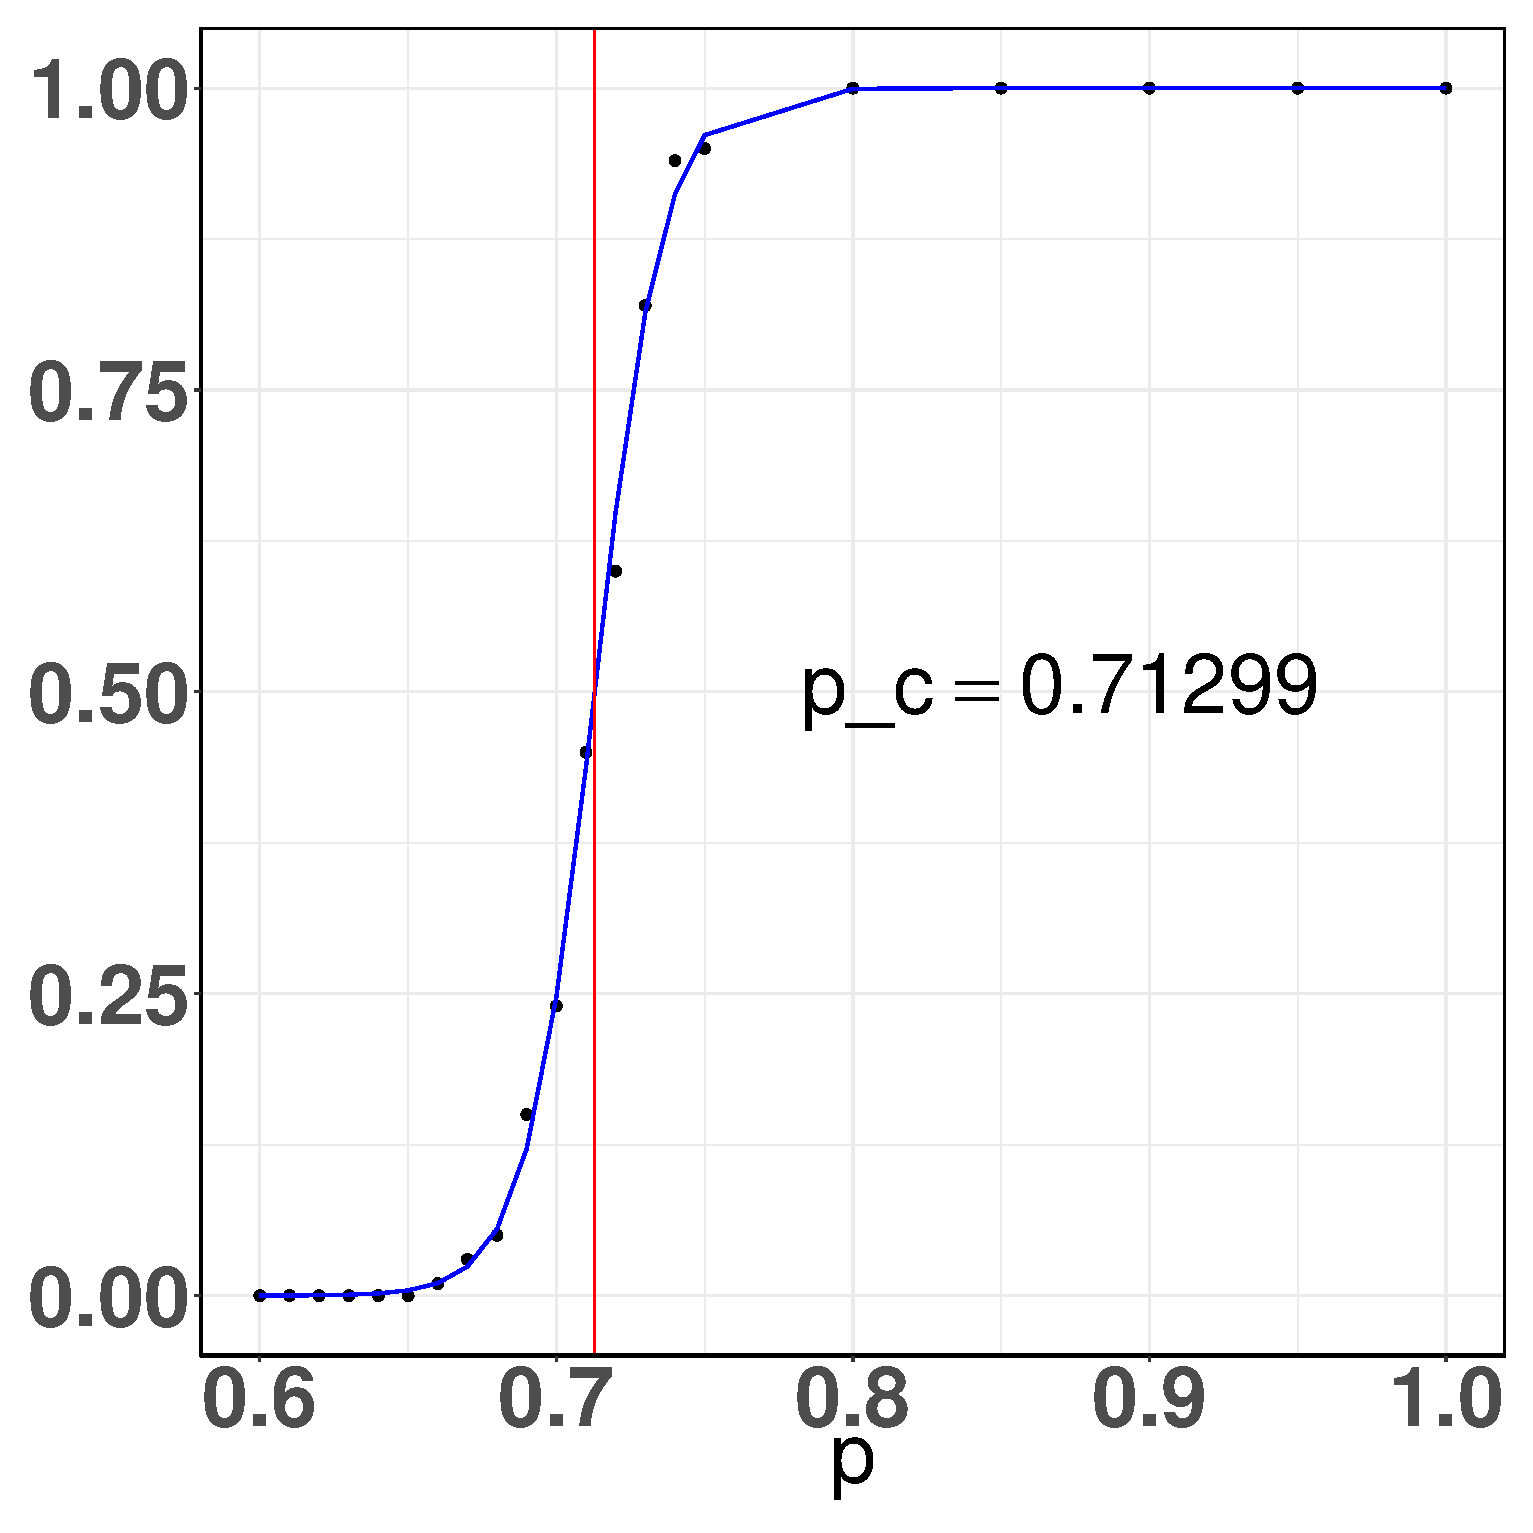
\includegraphics[width=0.48\textwidth]{Site-threshold-PVT}}\hfill
\subcaptionbox{Estimation of $H \mapsto U_c(H)$ \label{fig:thresholdsite+Uc(H)b}}{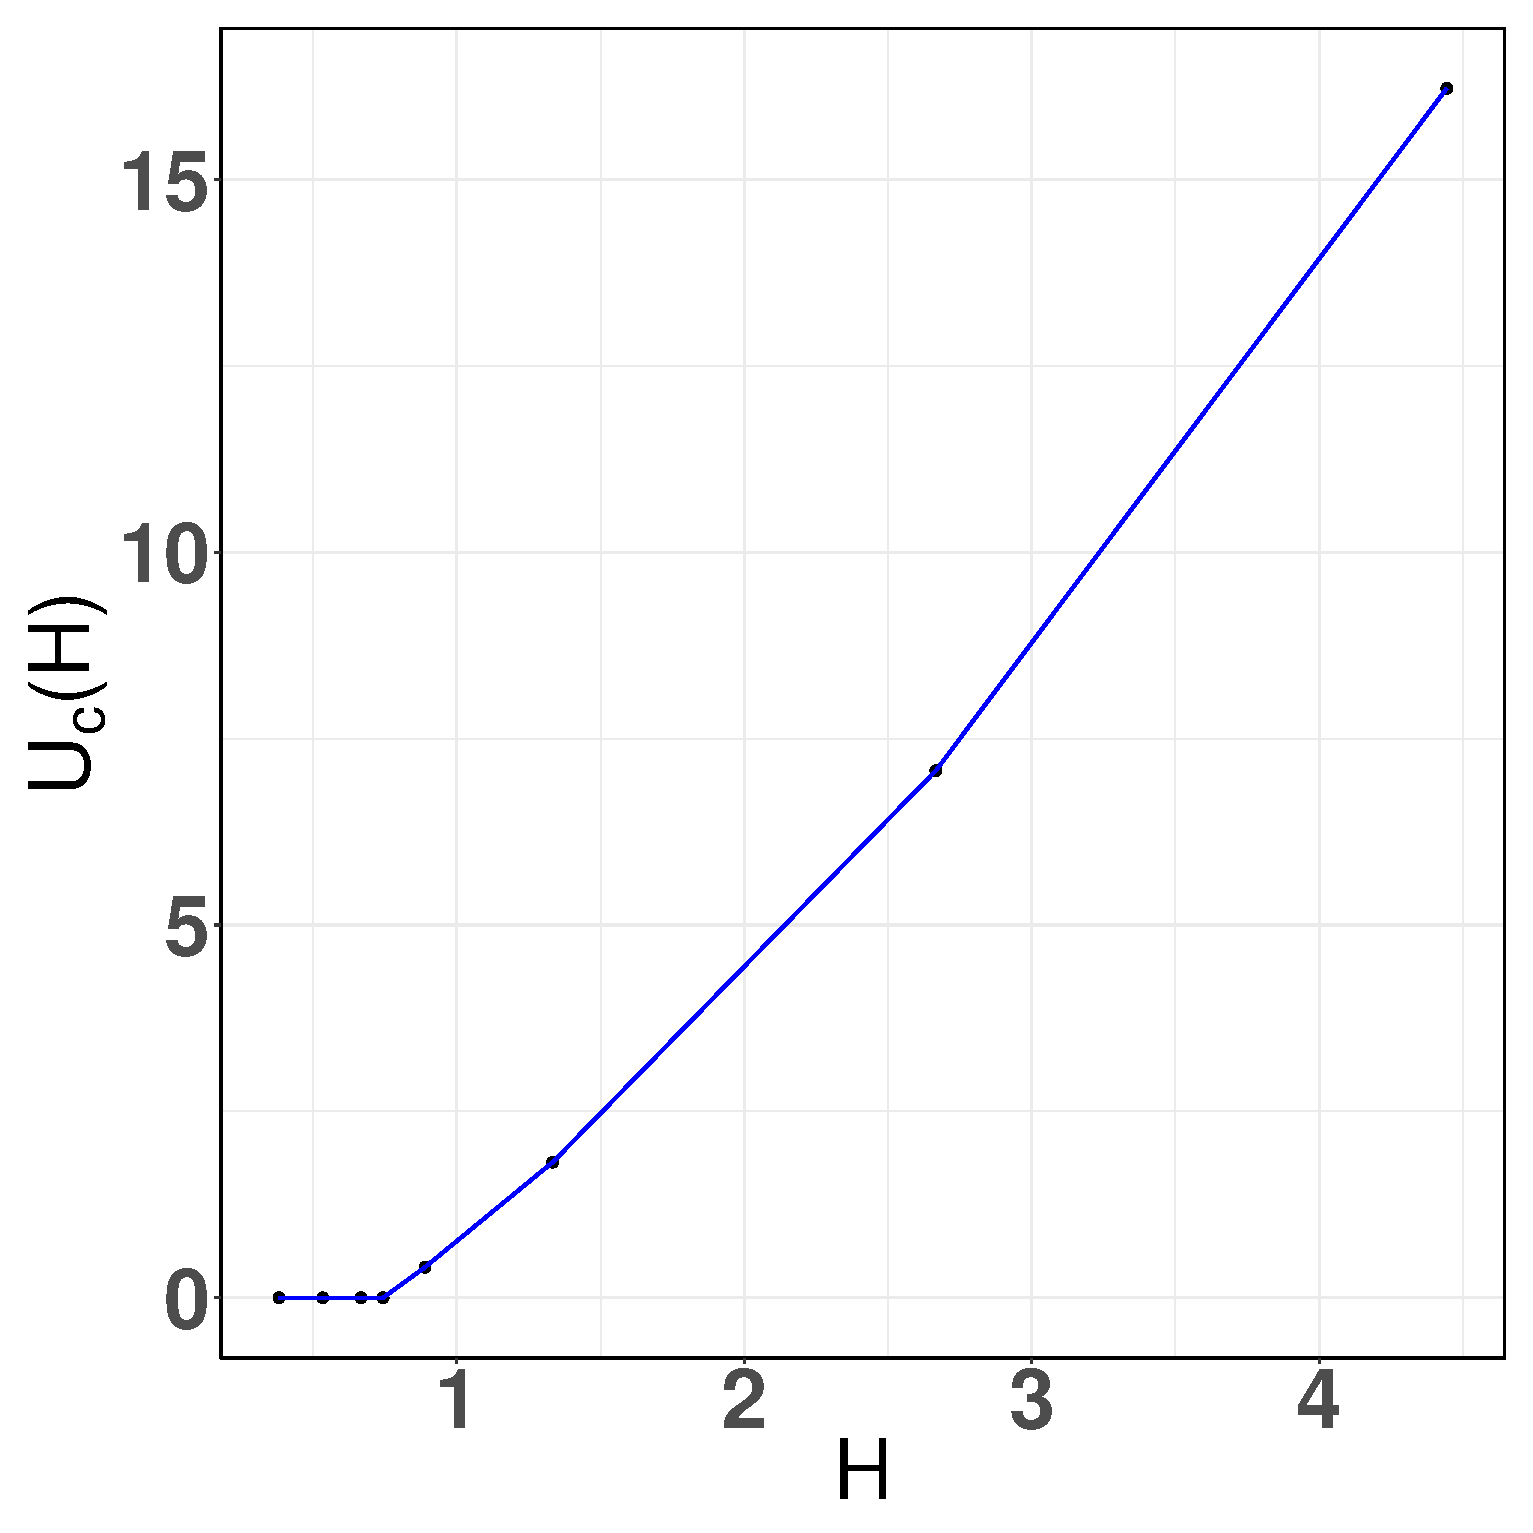
\includegraphics[width=0.48\textwidth]{Uc-general-curve}}\hfill
\caption{Numerical estimations of the Voronoi site percolation threshold $p^*$ and of the function $H \mapsto U_c(H)$ given by Theorem~\ref{Thm.analogue:subcritical}} \label{fig:thresholdsite+Uc(H)}
\end{figure}
Figure~\ref{fig:thresholdsite+Uc(H)a} shows an estimation of the critical value of the Bernoulli parameter $p^*=p_c$. We obtained the following estimate: $p^* \approx 0.71299$, very close to the numerical estimates given in~\cite{becker_percolation_2009,neher2008topological}. \\

The former observations lead to several related questions which we only were able to solve numerically:
\begin{enumerate}
    \item When $H$ is chosen sufficiently small so as to have $U_c(H)=0$, it means that percolation is solely ensured by the Bernoulli process. We then know that $\mathcal{G}_{1,0,H}$ percolates with positive probability. Then, is there a non trivial critical parameter $p^*<p<1$ above which percolation  of $\mathcal{G}_{p,0,H}$ still occurs with positive probability?
    \item Can we estimate $H_0$, the threshold given by Theorem~\ref{Thm.analogue:subcritical}?
    \item Can we estimate $U_c(p,H)$ when $p^* < p < 1$?
\end{enumerate}
\begin{figure}[h!]
\centering
\setlength{\lineskip}{\medskipamount}
\subcaptionbox{Estimation of $H \mapsto p_c(H)$\label{fig:additionalquestionsa}}{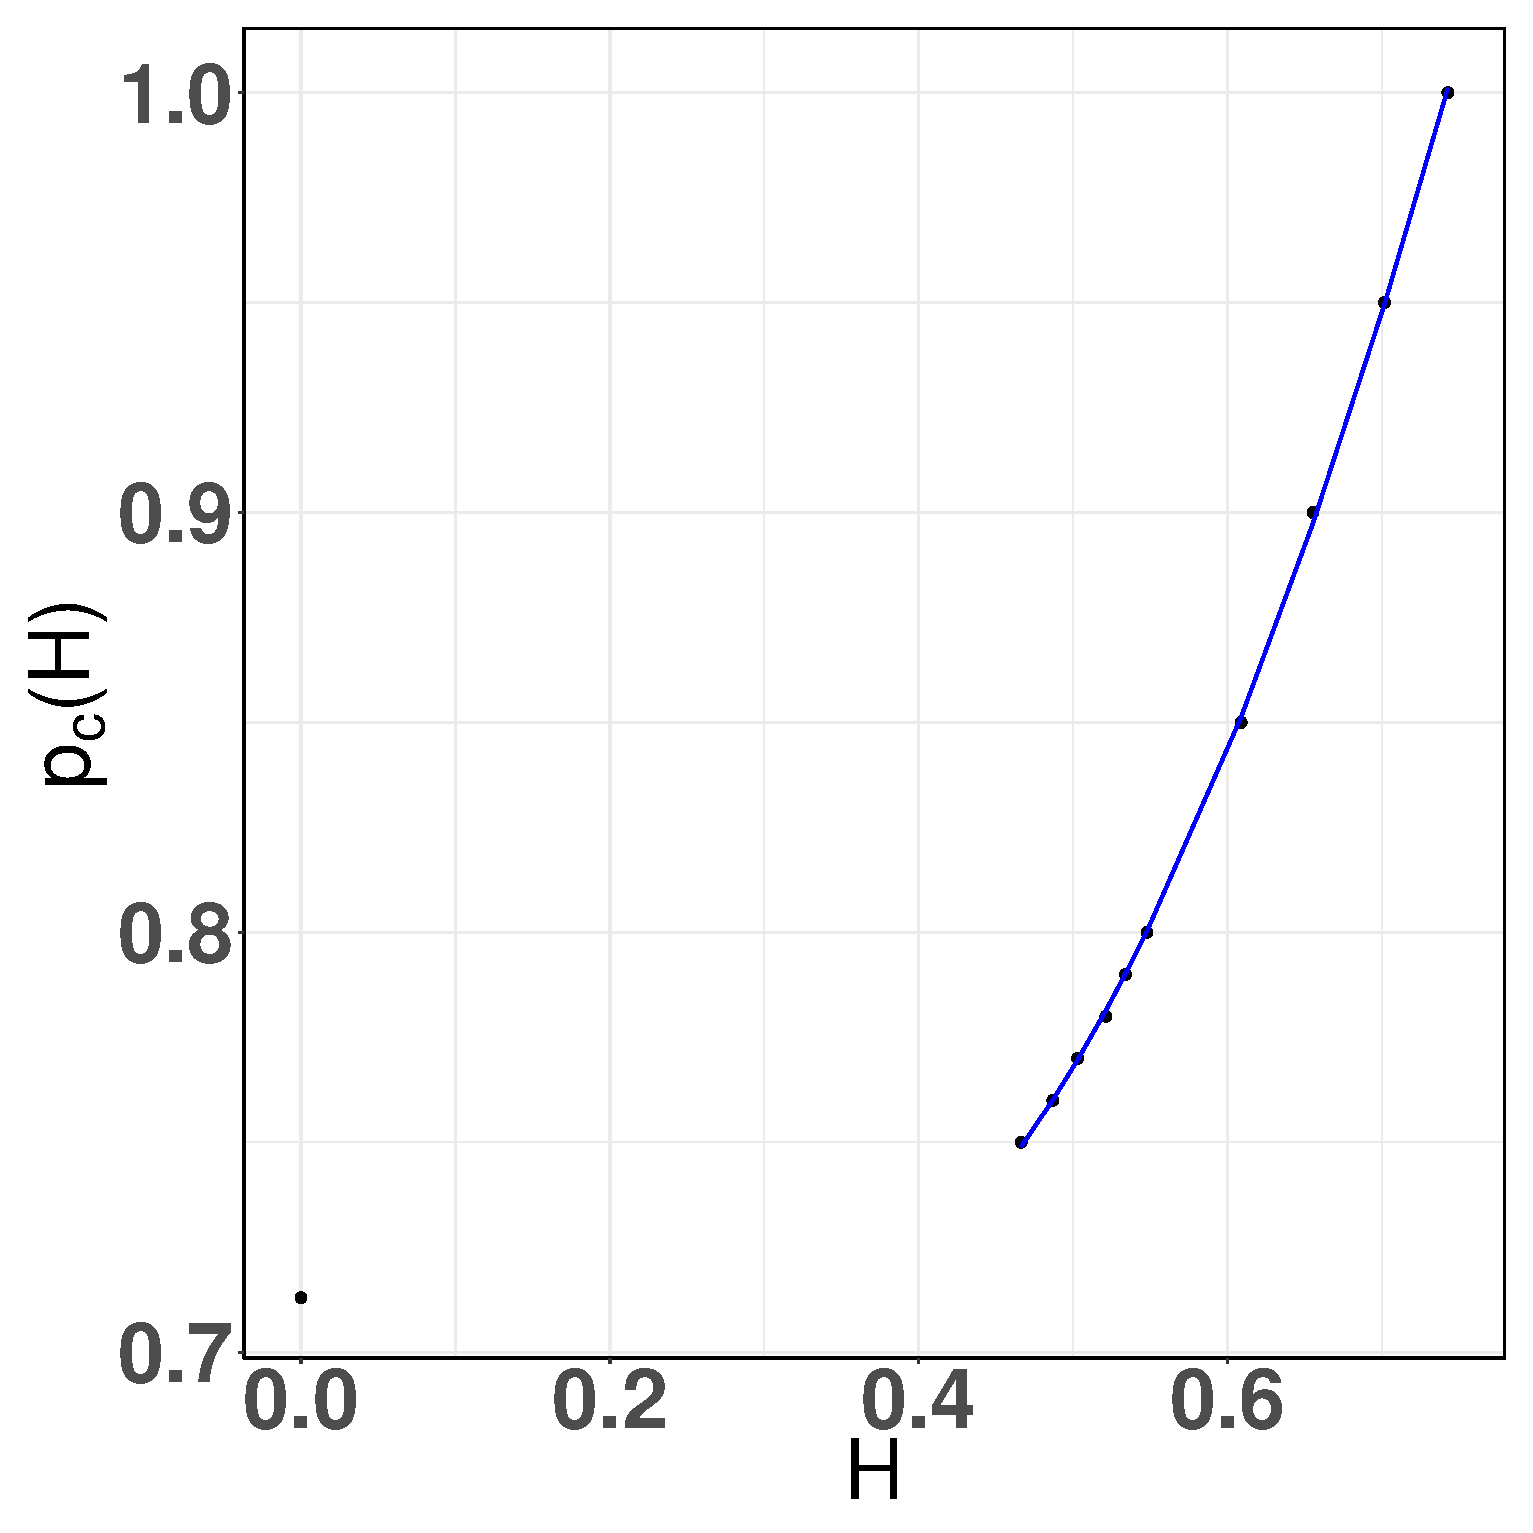
\includegraphics[width=0.48\textwidth]{pcH}}\hfill
\subcaptionbox{Estimation of $(p,H) \mapsto U_c(p,H)$ \label{fig:additionalquestionsb}}{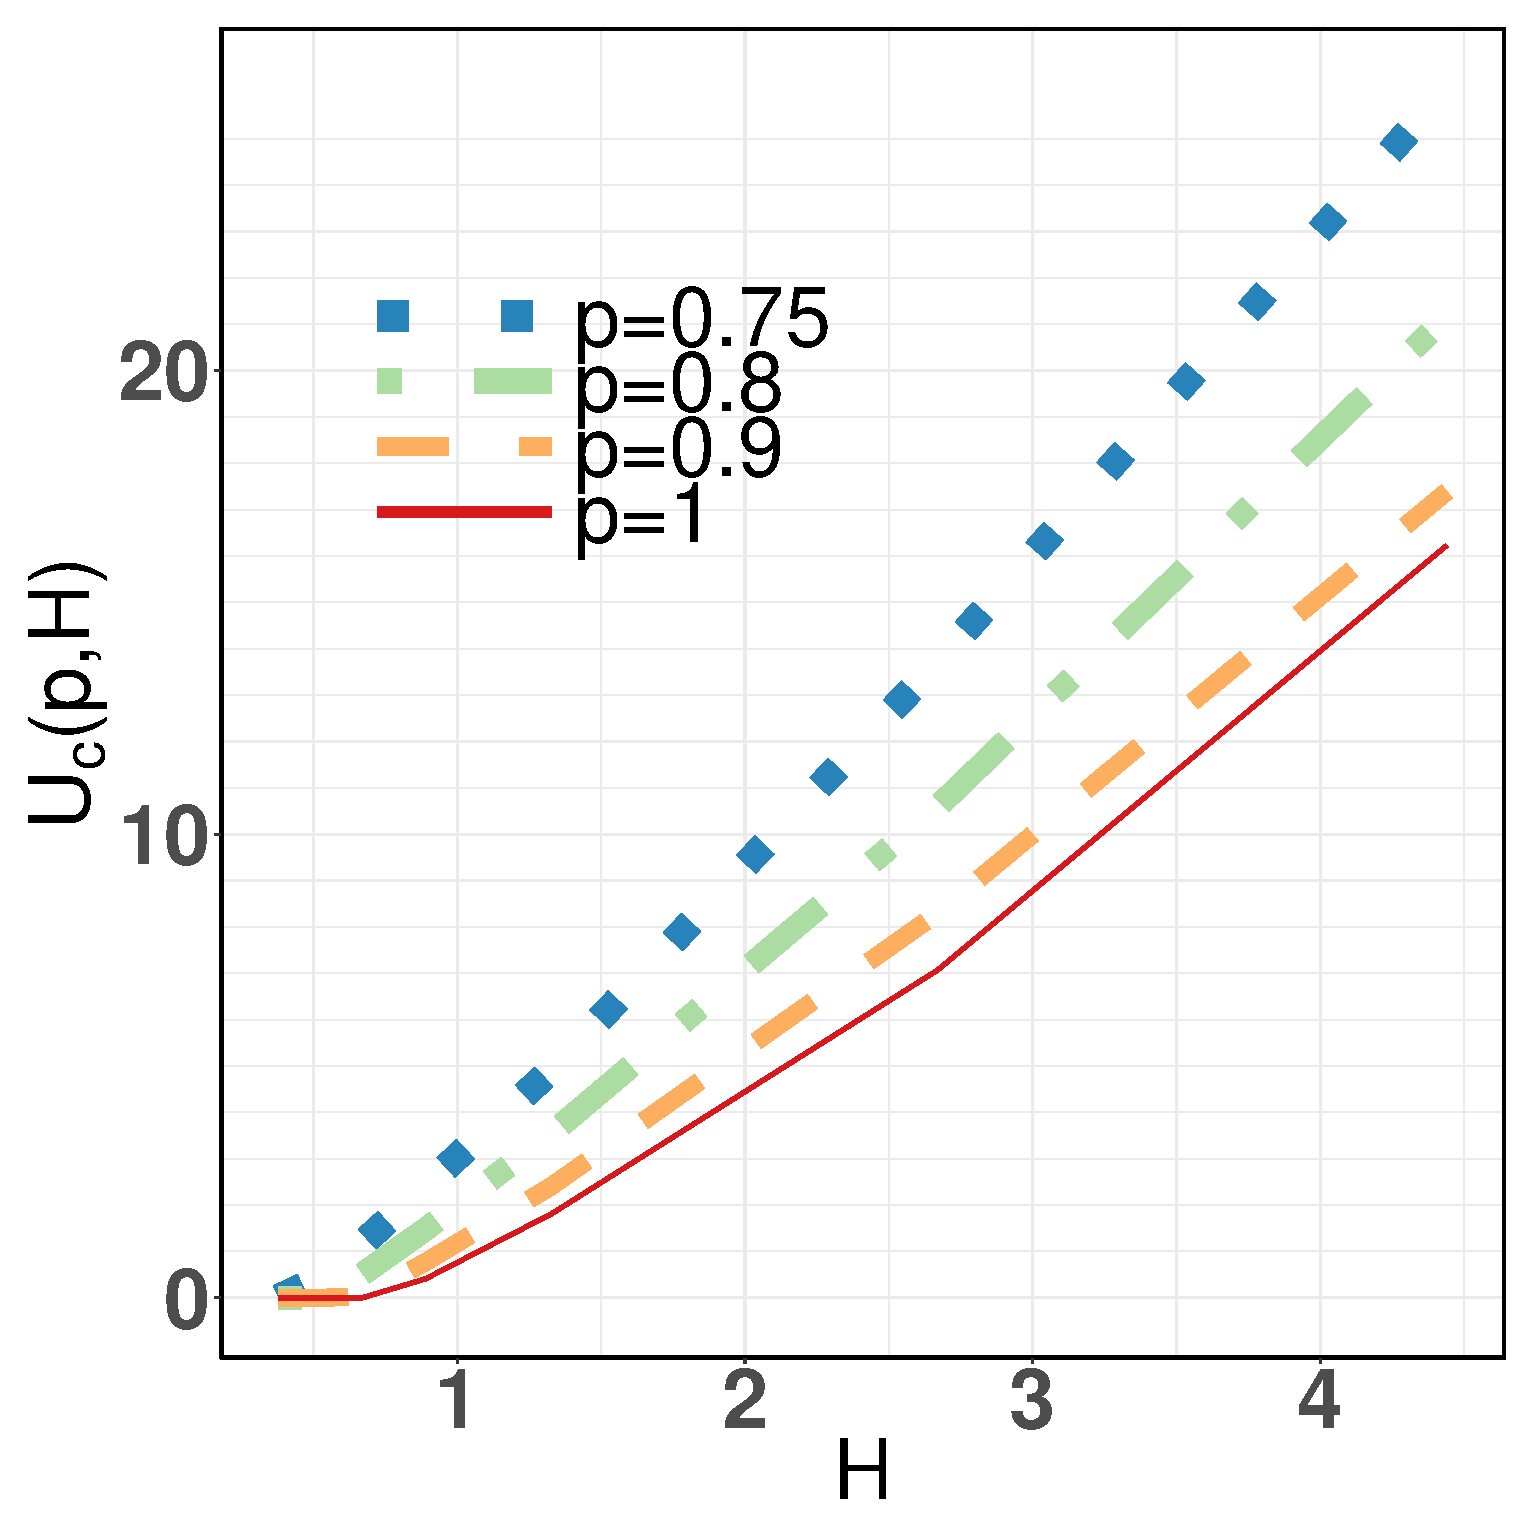
\includegraphics[width=0.48\textwidth]{critical-U-several-p}}\hfill
\caption{Numerical estimations of the critical parameter $p_c(H)$ needed for percolation in the absence of Cox points and of the function $(p,H) \mapsto U_c(p,H)$ given by  Corollary~\ref{Coroll.analogue:subcritical}} \label{fig:additionalquestions}
\end{figure}
We indeed were able to numerically address the first and third aforementioned questions, see Figure~\ref{fig:additionalquestions}. \\
Figure~\ref{fig:additionalquestionsa} shows the numerical estimation for the critical parameter $p$ needed to ensure percolation in the absence of Cox points:
\begin{equation*}
    p_c(H) \coloneqq \inf \lbrace p > p^* \, : \, \mathbb{P}(\mathcal{G}_{p,0,H} \, \text{percolates} \, ) > 0 \rbrace
\end{equation*}
We only were able to estimate $p_c(H)$ for $H>0.46$. For smaller values of $H$, apart from the theoretical value $p_c(0)=p_c \approx 0.71299$, simulation becomes much trickier, as the system approaches criticality. A quadratic model $p_c(H) = aH^2+bH+c$ given by the blue curve provides a good fit. Figure~\ref{fig:additionalquestionsb} shows numerical estimations of $(p,H) \mapsto U_c(p,H)$. As is easily theoretically proven, $U_c(p,H)$ is decreasing in $p$ and increasing in $H$. \\
Regarding an approximation of $H_0$, the threshold given by Theorem~\ref{Thm.analogue:subcritical}, we proceeded as follows. Define first the following critical value for $H$:
\begin{equation*}
    H_c \coloneqq \sup \lbrace H > 0, \, \mathbb{P}(\mathcal{G}_{1,0,H} \text{ percolates}) >0 \rbrace
\end{equation*}
If $H_c > 0$, then it is possible to have percolation of the connectivity graph when all crossroads are equipped with relays, i.e. $\mathbb{P}(\mathcal{G}_{1,0,H} \text{ percolates}) > 0$. Figure~\ref{fig:Hc} illustrates the result of our Monte-Carlo simulations and the estimation  $H_c \approx 0.743$.

\begin{figure}[ht!]
    \centering
    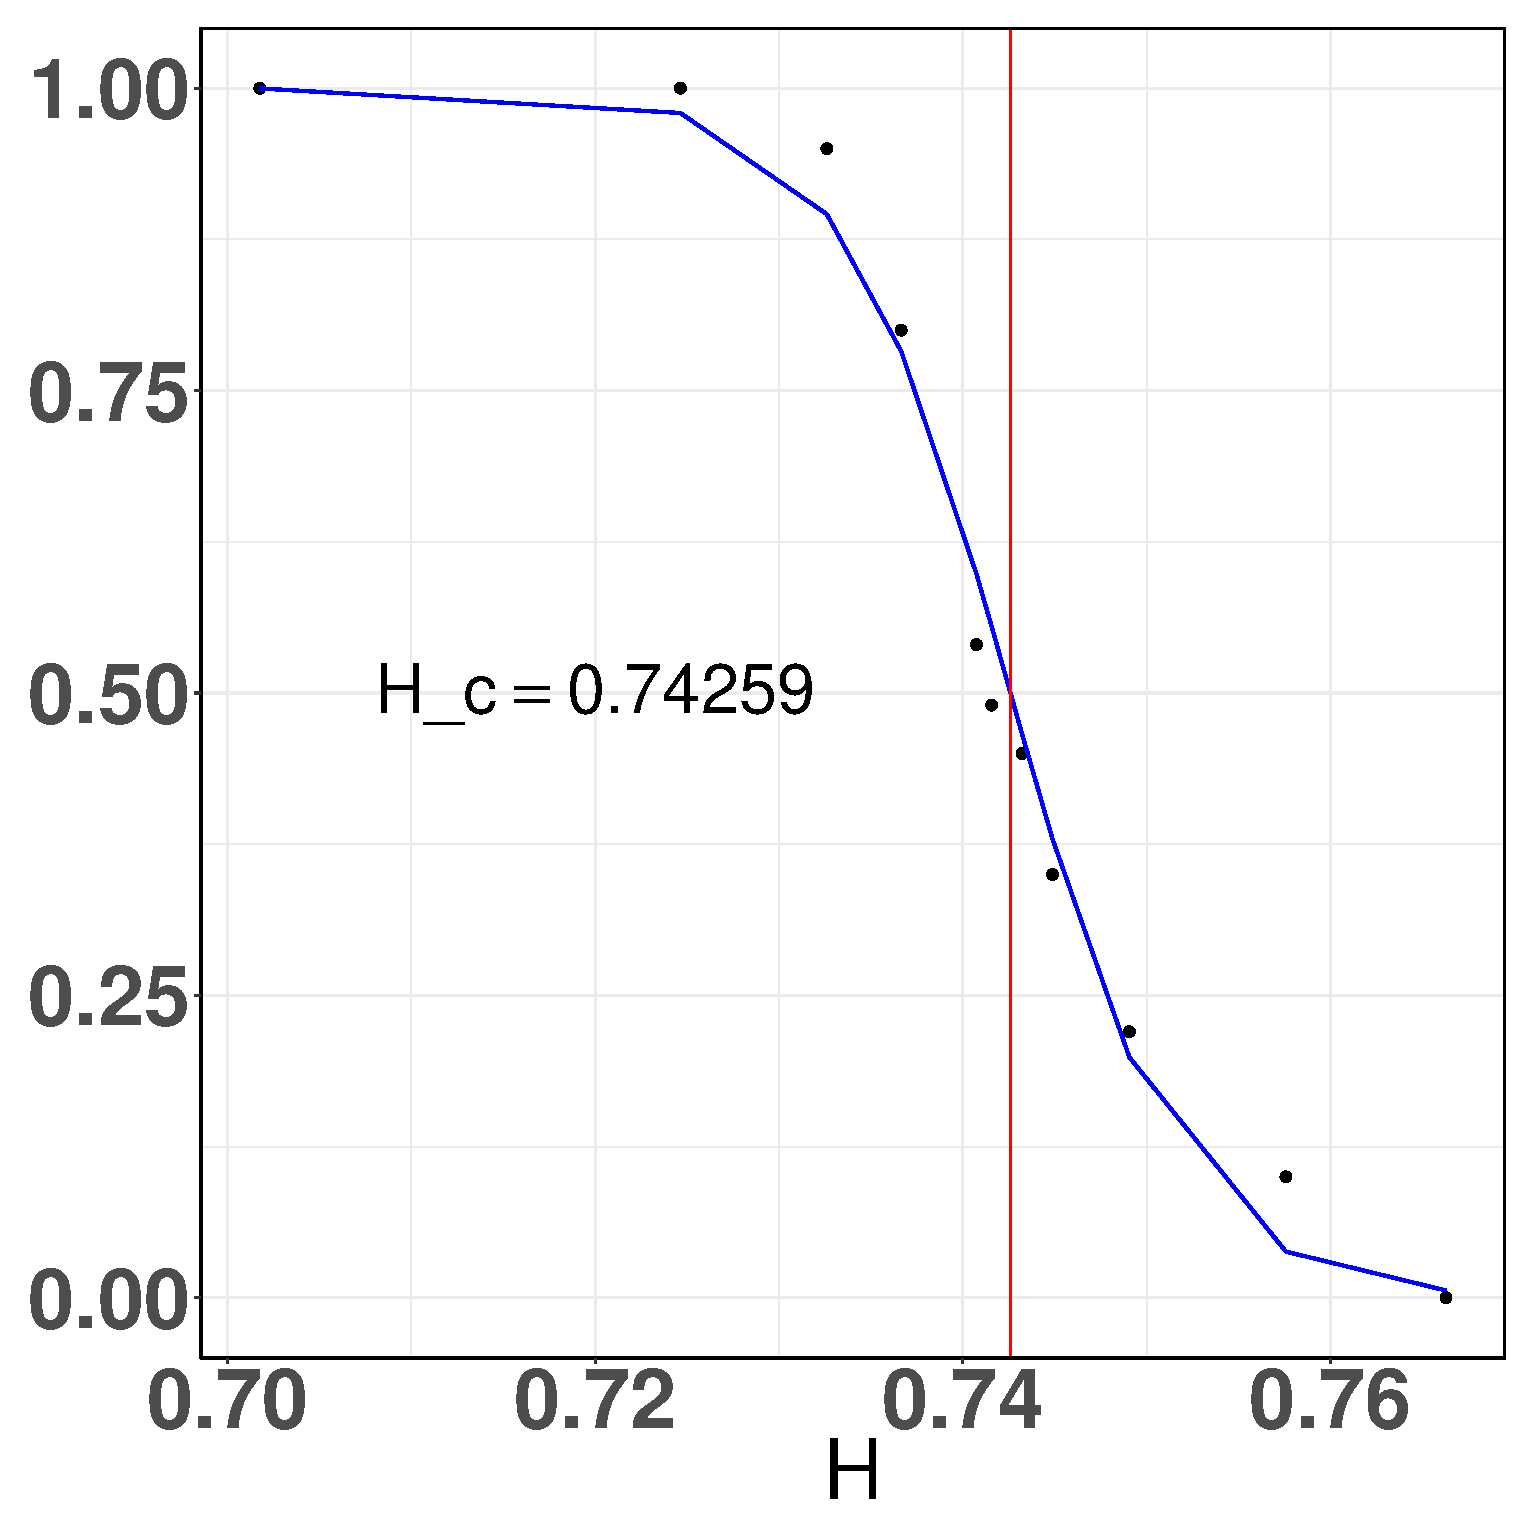
\includegraphics[scale=0.21]{sites-H_c-p=1}
    \caption{Numerical estimation of $H_c$}
    \label{fig:Hc}
\end{figure}

\noindent From the definition of $H_c$ and Theorem~\ref{Thm.analogue:subcritical}, it is clear that $H_0 \geq H_c$. Our simulations moreover suggest that $p_c(H_c)\approx 1$ and that $H_0 \approx H_c$ and we therefore conjecture that $H_0 \approx H_c$, thus estimating $H_0 \approx 0.743$. Matching theoretical results are tracks to follow for future work.

%We finally obtained the numerical estimate for the threshold $H_c$ above which all crossroads have to be endowed with a Bernoulli point: $p_c(H_c) = 1 \Leftrightarrow H_c \approx 0.743$. Note that we can also define $H_c$ in the following way:
%This also partially answers the second aforementioned question: our simulations suggest that $H_0 \approx H_c$. However, we were not able to prove this with rigorously. 
%there is a possible theoretical gap (due to the fact that the percolation function $\theta$ may not be continuous) %as an analogy consider the fact that
%which we were not able to quantify between $H_c$ and the critical value $H_0$ given by Theorem~\ref{Thm.subcritical}. However, our simulations suggest that $H_0 \approx H_c$. A matching theoretical result is a track to follow for future work. %say that theta function may not be continuous, which explains the gap.

\newpage
\section{Concluding remarks}
\label{S.Conclusion}

In this paper, we have introduced and studied a new model for continuum LOS percolation in a random environment. This mathematical model can be seen as a good candidate for the modelling of telecommunications networks in an urban scenario with regular obstructions: the random support (equivalent to the street system of the city) is modelled by a PVT. Users are dropped on the edges of the PVT (i.e. the streets of the city) according to a Cox point process with linear intensity $\lambda$. Obstructive connectivity conditions require the presence of an additional Bernoulli point process (representing relays which could either be real users or physical antennas) at the vertices of the PVT (crossroads of the city) to ensure connectivity between adjacent streets. We have proven that a minimal relay proportion $p > p_c$ is necessary to allow for percolation of the connectivity graph, that a non-trivial subcritical phase exists whenever the connectivity threshold $r$ is not too large and that a supercritical phase exists for all $r>0$. To prove these theoretical statements, we appealed to renormalisation techniques and stochastic geometry tools, as customary in any continuum percolation approach. Moreover, we also performed Monte-Carlo simulations to get numerical estimations of critical parameters of our model. \\
\indent Our results can easily be generalised to the \emph{dual tessellation} of a PVT: a \emph{Poisson-Delaunay} tessellation \cite[Section 9.2]{chiu_stochastic_2013}. %This is due to the fact that the dual tessellation is obtained by taking the center of each cell of the original tessellation as a vertex and by joining the centers of adjacent cells.
For the purpose of conciseness, we also assumed the random support of the Cox process to be a sufficiently regular tessellation, but we believe that our results are still valid for any stabilizing and essentially asymptotically connected tessellation as defined in Definitions~\ref{Def.stabilizing} and~\ref{Def.eac}. Finally, another stream of generalization could be to investigate the case of higher dimensions, which we omitted to do as it is physically less relevant. \\
\indent Our approach paves the way to the study of new continuum percolation models where two connection radii could appear: one for LOS connections (i.e. nodes of the network being located on the same edge of the random support) and one for non-line-of-sight (NLOS) connections (i.e. nodes of the network being located on different edges of the random support). This interesting generalization of Gilbert's original continuum percolation model, of interest for more realistic models of telecommunications networks, has not been studied yet, as far as we know.
\bibliographystyle{amsplain}
\bibliography{references}


\end{document} 

